\documentclass[11pt,a4paper]{article}

\usepackage[utf8]{inputenc}
\usepackage[T1]{fontenc}
\usepackage{amsmath,amssymb}
\usepackage{graphicx}
\usepackage{booktabs}
\usepackage{hyperref}
\usepackage[margin=1in]{geometry}
\usepackage{caption}
\usepackage{subcaption}
\usepackage{float}
\usepackage{xcolor}
\usepackage{xspace}

%%% Custom commands %%%
\newcommand{\ET}{\ensuremath{E_{\text{T}}}\xspace}
\newcommand{\eT}{\ensuremath{E_{\text{T}}}\xspace}
\newcommand{\pT}{\ensuremath{p_{\text{T}}}\xspace}
\newcommand{\etg}{\ensuremath{E_{\mathrm{T}}^{\gamma}}\xspace}
\newcommand{\isoET}{\mbox{$E_{\text{T}}^{\text{iso}}$}\xspace}
\newcommand{\isoETtruth}{\ensuremath{E_\text{T}^\text{iso,truth}}\xspace}
\newcommand{\wetacog}{\ensuremath{w_{\eta}^{\mathrm{CoG}}}\xspace}
\newcommand{\chidf}{\ensuremath{\chi^2/\mathrm{ndf}}\xspace}
\newcommand{\DR}{\ensuremath{\Delta R}\xspace}
\newcommand{\zvtx}{\ensuremath{z_{\mathrm{vtx}}}\xspace}
\newcommand{\pp}{\mbox{$p$+$p$}\xspace}
\newcommand{\GeV}{\ifmmode {\mathrm{\ Ge\kern -0.1em V}}\else\textrm{Ge\kern -0.1em V}\fi\xspace}

\title{\LARGE\textbf{Updates Since Preliminary Result:\\
BDT, NPB Removal, Double Interactions,\\
and Shower Shape Comparisons}}
\author{PPG12 Analysis Team (automated report)}
\date{April 9, 2026}

\begin{document}

\maketitle

\begin{abstract}
This report summarizes the major analysis updates implemented since the
preliminary isolated photon cross-section result in \pp collisions at
$\sqrt{s} = 200$~\GeV with sPHENIX Run~24 data.
Four work streams are covered:
(1)~the photon identification BDT, expanded from a minimal feature set to
11 model variants with an $\ET$-dependent parametric threshold;
(2)~non-physics background (NPB) rejection, upgraded from a hard timing cut
to a dedicated 25-feature XGBoost score;
(3)~double-interaction efficiency studies, demonstrating that the apparent
reconstruction efficiency drop in pileup MC is a truth--reco matching artifact;
and (4)~shower shape data--MC comparisons using pileup-blended MC templates,
which improve \chidf by factors of up to $22\times$.
Each section documents the methodology, key results, and implications for the
cross-section measurement.
\end{abstract}

\tableofcontents
\clearpage

%% =================================================================
\section{Introduction}
\label{sec:intro}

The PPG12 isolated photon cross-section measurement uses sPHENIX Run~24 \pp
data at $\sqrt{s} = 200$~\GeV with an integrated luminosity of 16.6~pb$^{-1}$
(1.5~mrad crossing-angle period, runs 51274--54000).
The measurement employs the ABCD double-sideband method for background
subtraction, with photon identification based on electromagnetic shower shape
variables evaluated by a Boosted Decision Tree (BDT), and topological cluster
isolation with $R = 0.4$.
Twelve \eT bins span 8--35~\GeV within $|\eta| < 0.7$.

Since the preliminary result, four areas have undergone substantial development:
\begin{enumerate}
    \item \textbf{BDT photon identification} (\S\ref{sec:bdt}): Feature expansion,
      model variant studies, parametric threshold, and systematic framework.
    \item \textbf{NPB rejection} (\S\ref{sec:npb}): New dedicated XGBoost model
      replacing the hard timing preselection.
    \item \textbf{Double-interaction efficiency} (\S\ref{sec:double_eff}):
      Decomposition of the pileup efficiency drop into matching artifact vs.\
      genuine physics effects.
    \item \textbf{Shower shape comparisons} (\S\ref{sec:showershape}): Pileup-blended
      MC templates and quantitative data--MC agreement assessment.
\end{enumerate}


%% =================================================================
\section{BDT Photon Identification}
\label{sec:bdt}

\subsection{Feature Expansion}
\label{subsec:bdt_features}

The preliminary BDT used a minimal feature set of 6 variables: cluster \ET,
$\eta$, $\phi$, vertex $z$, $E_{1\times1}/E_{3\times3}$, and $E_{3\times2}/E_{3\times5}$.
The updated analysis expands the training feature space to 25 variables, adding
tower energy fractions, cluster width moments, and a broader set of energy
ratios:

\begin{itemize}
    \item \textbf{Tower energy fractions}: $e_{t1} = (E_1{+}E_2{+}E_3{+}E_4)/E_{\text{tot}}$,
      $e_{t2}$, $e_{t3}$, $e_{t4}$ (quadrant asymmetries)
    \item \textbf{Cluster width moments}: $w_\eta^{\text{CoG}}$ (eta width),
      $w_\phi^{\text{CoG}}$ (phi width), $w_{3\times2}$, $w_{5\times2}$, $w_{7\times2}$
    \item \textbf{Energy ratios}: $E_{1\times1}/E_{2\times2}$,
      $E_{1\times1}/E_{1\times3}$, $E_{1\times1}/E_{1\times5}$,
      $E_{1\times1}/E_{1\times7}$, $E_{1\times1}/E_{3\times1}$,
      $E_{1\times1}/E_{5\times1}$, $E_{1\times1}/E_{7\times1}$,
      $E_{2\times2}/E_{3\times3}$, $E_{2\times2}/E_{3\times5}$,
      $E_{2\times2}/E_{3\times7}$, $E_{2\times2}/E_{5\times3}$
\end{itemize}

Training uses \textsc{pythia-8} photon MC (photon5/10/20, truth pid $\in \{1,2\}$)
as signal and jet MC (jet10/15/20/30/50, pid $\notin \{1,2\}$) as background,
with $6 < \ET < 40$~\GeV and $|\eta| < 0.7$.

\subsection{Model Variants}
\label{subsec:bdt_variants}

To study feature importance and optimize the trade-off between discrimination
power and robustness, 11 model variants are trained via systematic feature
ablation:

\begin{table}[H]
    \centering
    \caption{BDT model variants defined by feature subsets. All variants include
      vertex $z$, $\eta$, $E_{1\times1}/E_{3\times3}$, and $e_{t1}$--$e_{t4}$ as
      baseline features. The ``E'' suffix denotes variants that include cluster
      \ET as an explicit feature.}
    \label{tab:bdt_variants}
    \begin{tabular}{llcl}
        \toprule
        Variant & Additional features & Count & Purpose \\
        \midrule
        \texttt{base}      & (baseline only) & 7 & Minimal reference \\
        \texttt{base\_vr}  & (vertex-reweighted) & 7 & Vertex robustness check \\
        \texttt{base\_v0}  & Drops $e_{t1}$ & 6 & Remove isolation-correlated feature \\
        \texttt{base\_v1}  & $+\,w_\eta^{\text{CoG}}$ & 8 & Add width \\
        \texttt{base\_v2}  & $+\,w_\eta^{\text{CoG}},\,w_\phi^{\text{CoG}}$ & 9 & Add 2D shape \\
        \texttt{base\_v3}  & $+\,w_\eta^{\text{CoG}},\,w_\phi^{\text{CoG}},\,E_{3\times2}/E_{3\times5}$ & 10 & Full shape \\
        \texttt{base\_E}   & $+\,\ET$ & 8 & Energy-aware base \\
        \texttt{base\_v0E} & $+\,\ET$, drops $e_{t1}$ & 7 & Energy + iso-insensitive \\
        \texttt{base\_v1E} & $+\,\ET,\,w_\eta^{\text{CoG}}$ & 9 & \textbf{Nominal} \\
        \texttt{base\_v2E} & $+\,\ET,\,w_\eta^{\text{CoG}},\,w_\phi^{\text{CoG}}$ & 10 & Energy + 2D shape \\
        \texttt{base\_v3E} & $+\,\ET,\,w_\eta^{\text{CoG}},\,w_\phi^{\text{CoG}},\,E_{3\times2}/E_{3\times5}$ & 11 & Full feature set \\
        \bottomrule
    \end{tabular}
\end{table}

The nominal analysis uses \texttt{base\_v1E} (9 features) in both \ET bins
$[8, 15]$ and $[15, 35]$~\GeV, with \texttt{base\_E} as the default fallback.

\subsection{Training Procedure}
\label{subsec:bdt_training}

The XGBoost training applies three-stage reweighting to minimize kinematic
biases:
\begin{enumerate}
    \item \textbf{Class reweighting}: Balances signal and background counts.
    \item \textbf{\ET spectrum flattening}: Inverse-PDF spline reweighting to
      remove the steeply falling \ET spectrum, preventing the BDT from learning
      \ET-dependent shortcuts.
    \item \textbf{$\eta$ spectrum flattening}: Same procedure for the $\eta$
      distribution.
\end{enumerate}

Background subsampling is applied below $\ET = 15$~\GeV to address the
heavy-tail problem in the low-\ET region, using inverse-PDF reweighting across
20 \ET bins.

\begin{table}[H]
    \centering
    \caption{XGBoost hyperparameters for the photon identification BDT.}
    \label{tab:xgb_params}
    \begin{tabular}{lc}
        \toprule
        Parameter & Value \\
        \midrule
        Number of boosted trees & 750 \\
        Maximum depth & 5 \\
        Learning rate & 0.1 \\
        Subsample fraction & 0.5 \\
        Column sample per tree & 0.6 \\
        L1 regularization ($\alpha$) & 5.0 \\
        L2 regularization ($\lambda$) & 0.3 \\
        Grow policy & Loss-guided \\
        Tree method & Histogram-based \\
        \midrule
        Train / validation / test split & 70\% / 10\% / 20\% \\
        Random seed & 42 \\
        \bottomrule
    \end{tabular}
\end{table}

A split-sample approach divides MC into two independent halves to avoid
self-training bias: each half is scored by the model trained on the other half.
Models are exported via \texttt{TMVA::Experimental::SaveXGBoost} and applied in
the analysis via \texttt{TMVA::Experimental::RBDT::Compute()}.

\subsection{Training Performance}
\label{subsec:bdt_performance}

The nominal \texttt{base\_v1E} model achieves test-set AUC values of 0.88--0.93
across all \ET bins, evaluated on the 20\% held-out test sample with
cross-section-weighted events.  Table~\ref{tab:bdt_auc} summarizes the
per-bin performance; the best discrimination is in the 10--15~\GeV bin
(AUC~$= 0.925$), where the signal-to-background shower-shape contrast is
strongest, while the lowest AUC is at $6 < \ET < 10$~\GeV (0.884), where
fragmentation photons broaden the signal shower profiles.

\begin{table}[H]
    \centering
    \caption{Test-set AUC for the nominal \texttt{base\_v1E} BDT in each \ET
      training bin.  A single global model is trained on all bins simultaneously;
      the per-bin AUC is evaluated on the test split restricted to each \ET range.}
    \label{tab:bdt_auc}
    \begin{tabular}{lccccc}
        \toprule
        \ET bin [\GeV] & 6--10 & 10--15 & 15--20 & 20--25 & 25--35 \\
        \midrule
        Test AUC       & 0.884 & 0.925  & 0.911  & 0.914  & 0.912  \\
        Test events    & 591\,k & 658\,k & 442\,k & 389\,k & 125\,k \\
        \bottomrule
    \end{tabular}
\end{table}

Figures~\ref{fig:bdt_roc_split} and~\ref{fig:bdt_roc_nosplit} show the ROC
curves for all 11 photon-ID variants on the \texttt{CLUSTERINFO\_CEMC}
(split) and \texttt{CLUSTERINFO\_CEMC\_NO\_SPLIT} (nosplit) cluster nodes
respectively, with each panel showing the five \ET training bins as separate
curves.  The curves are well separated from the diagonal chance line across
the full false-positive-rate range, confirming that every variant provides
strong photon--jet discrimination in the high-\ET bins; the $6 < \ET <
10$~\GeV bin trails because signal photons at low \ET have poorer shower
resolution and the jet background is not yet kinematically suppressed.
The \texttt{base\_vr} panel is bit-identical to \texttt{base} (consistent with
the BDT-training audit's WARN-1: the ``vertex reweight'' variant config
accidentally does not enable \texttt{vertex\_reweight}, so the trained model
is a duplicate of \texttt{base}).  The \texttt{v0} and \texttt{v0E} variants,
which drop the dominant $e_{t1}$ feature, show the weakest discrimination.
AUCs in these plots are evaluated on a $\sim 590$\,k signal + bkg MC subset
drawn from \texttt{photon5/10/20} and \texttt{jet20/30} with $6 < \ET <
40$~\GeV and $|\eta| < 0.7$; absolute values therefore differ slightly from
the per-bin test-set AUCs quoted in Table~\ref{tab:bdt_auc} (which use the
training-time 20\% hold-out and class-balance-reweighted events), but the
ranking and shape of the curves are preserved.

\begin{figure}[H]
    \centering
    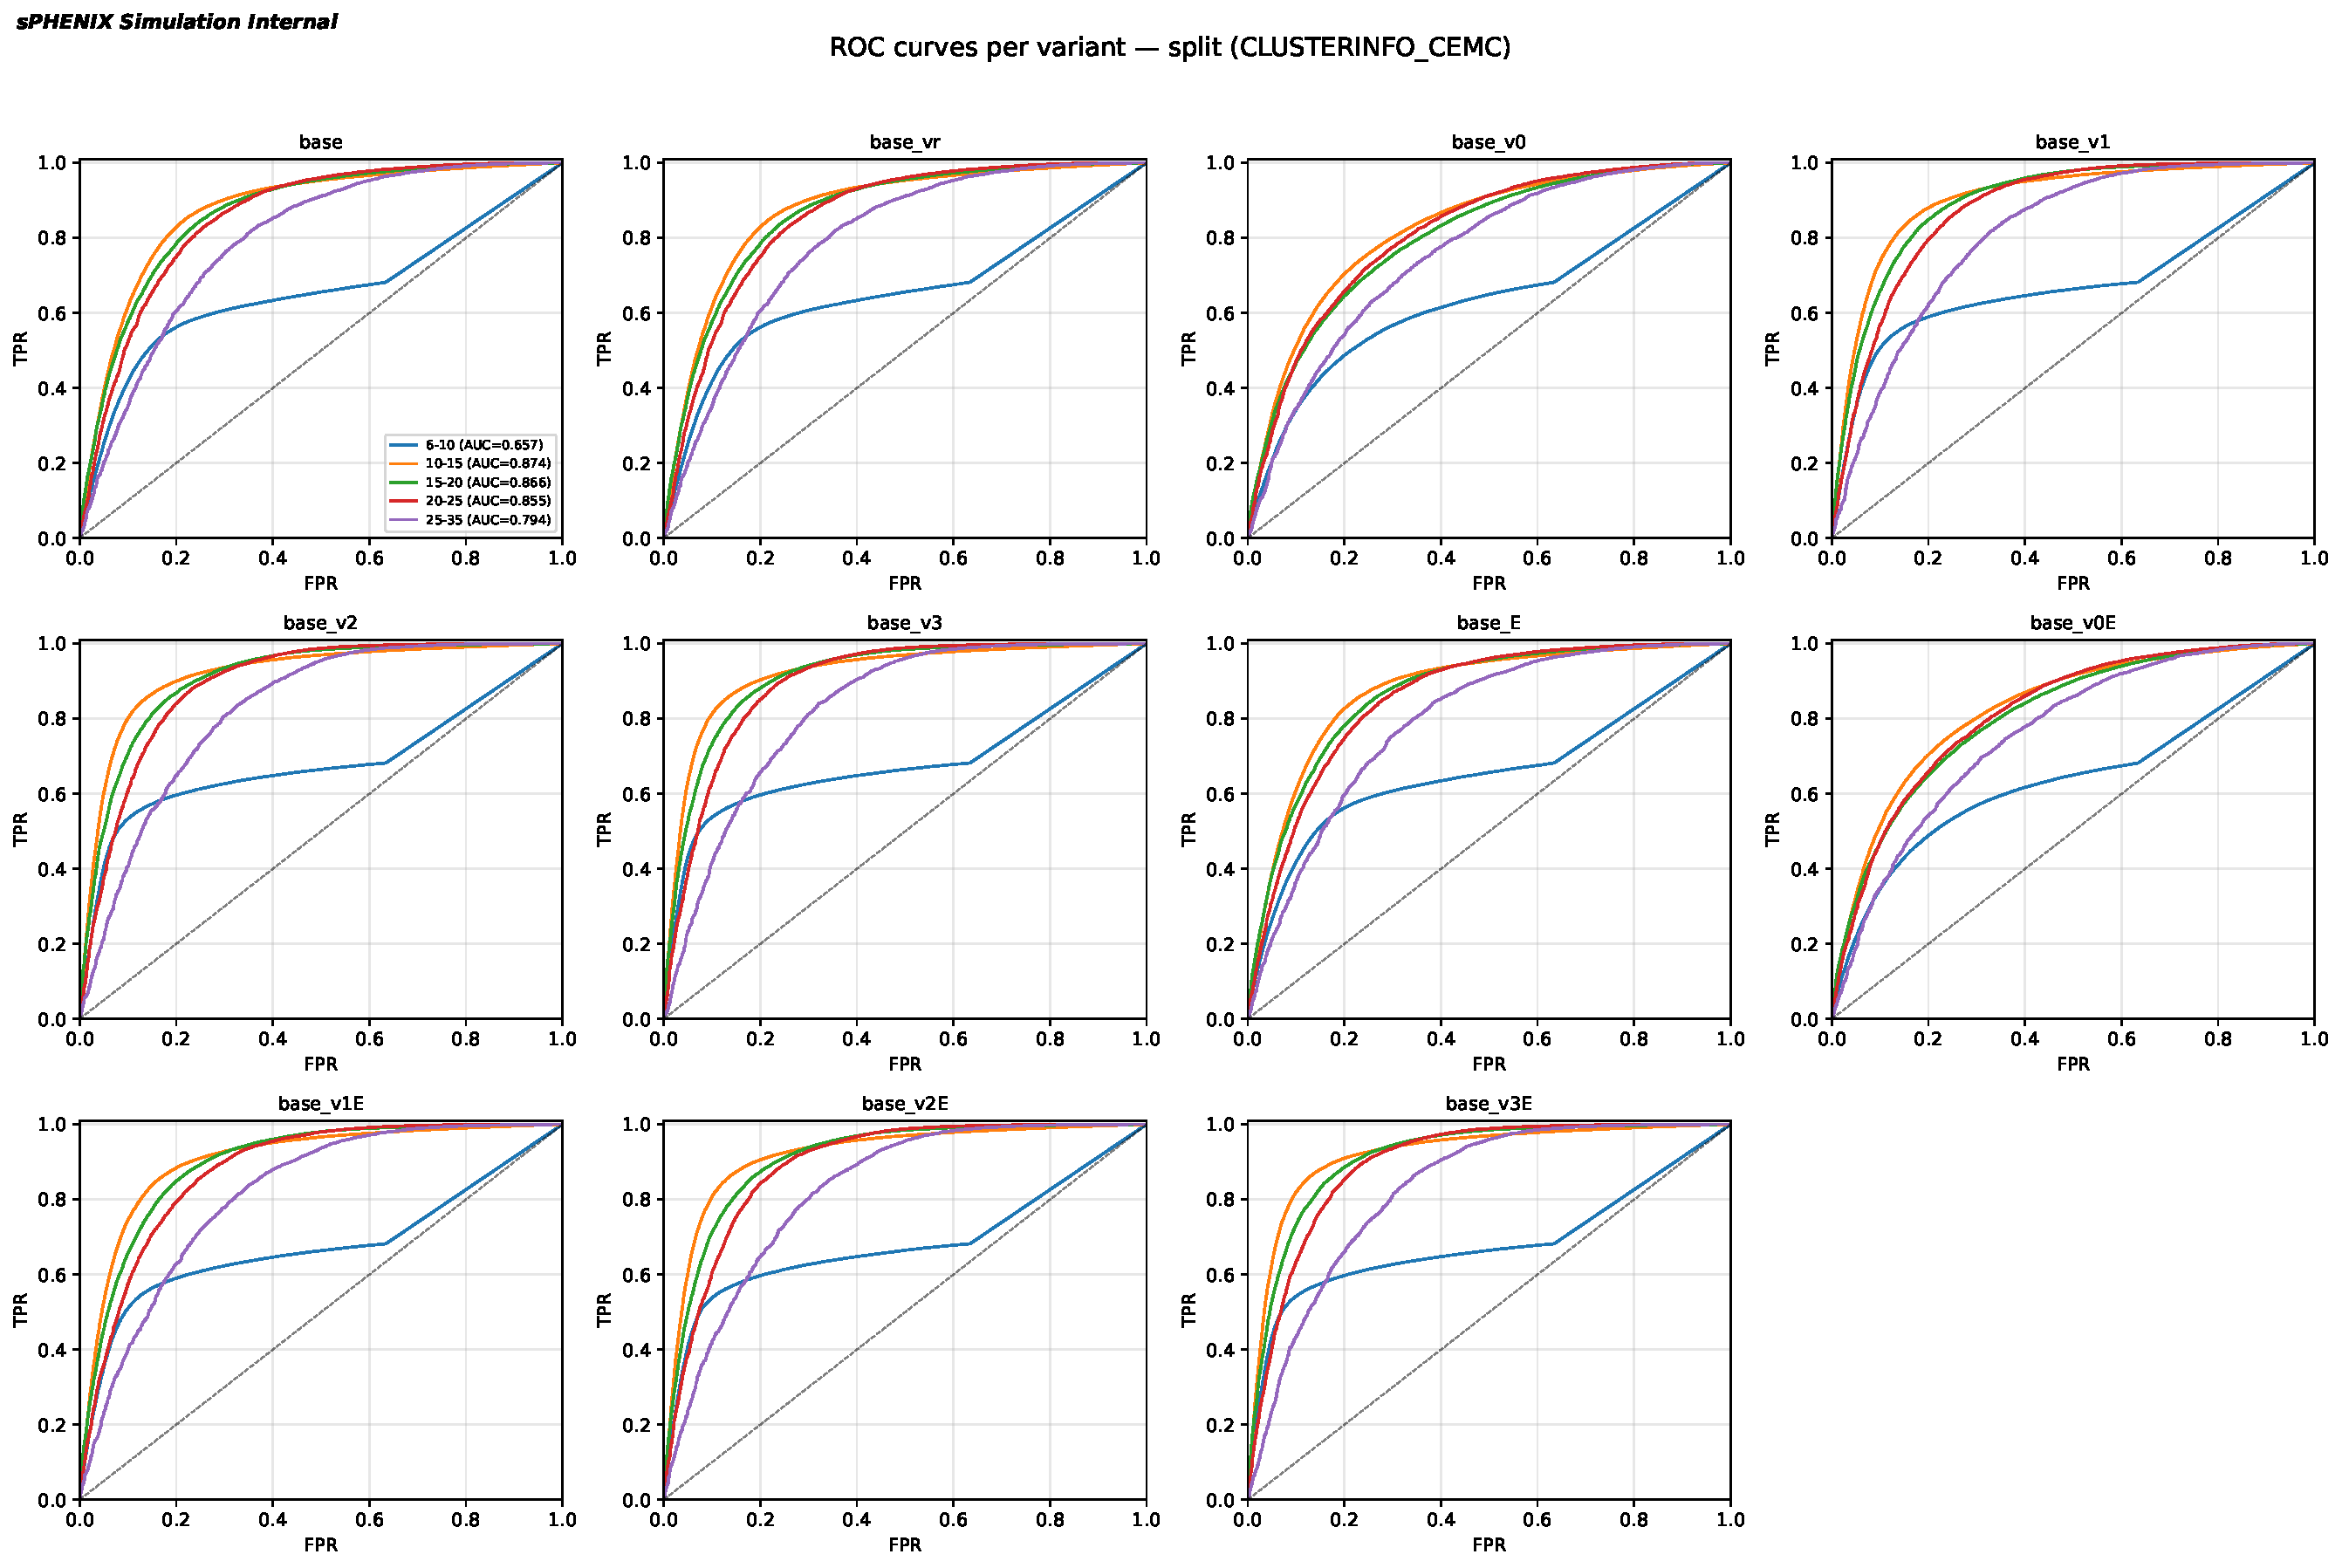
\includegraphics[width=\textwidth]{figures/bdt_audit/roc_grid_split.pdf}
    \caption{ROC curves for all 11 photon-ID variants on the split cluster
      node.  Each panel shows the five \ET training bins (colored curves,
      legend in the \texttt{base} panel).  The dashed line indicates
      chance-level discrimination.}
    \label{fig:bdt_roc_split}
\end{figure}

\begin{figure}[H]
    \centering
    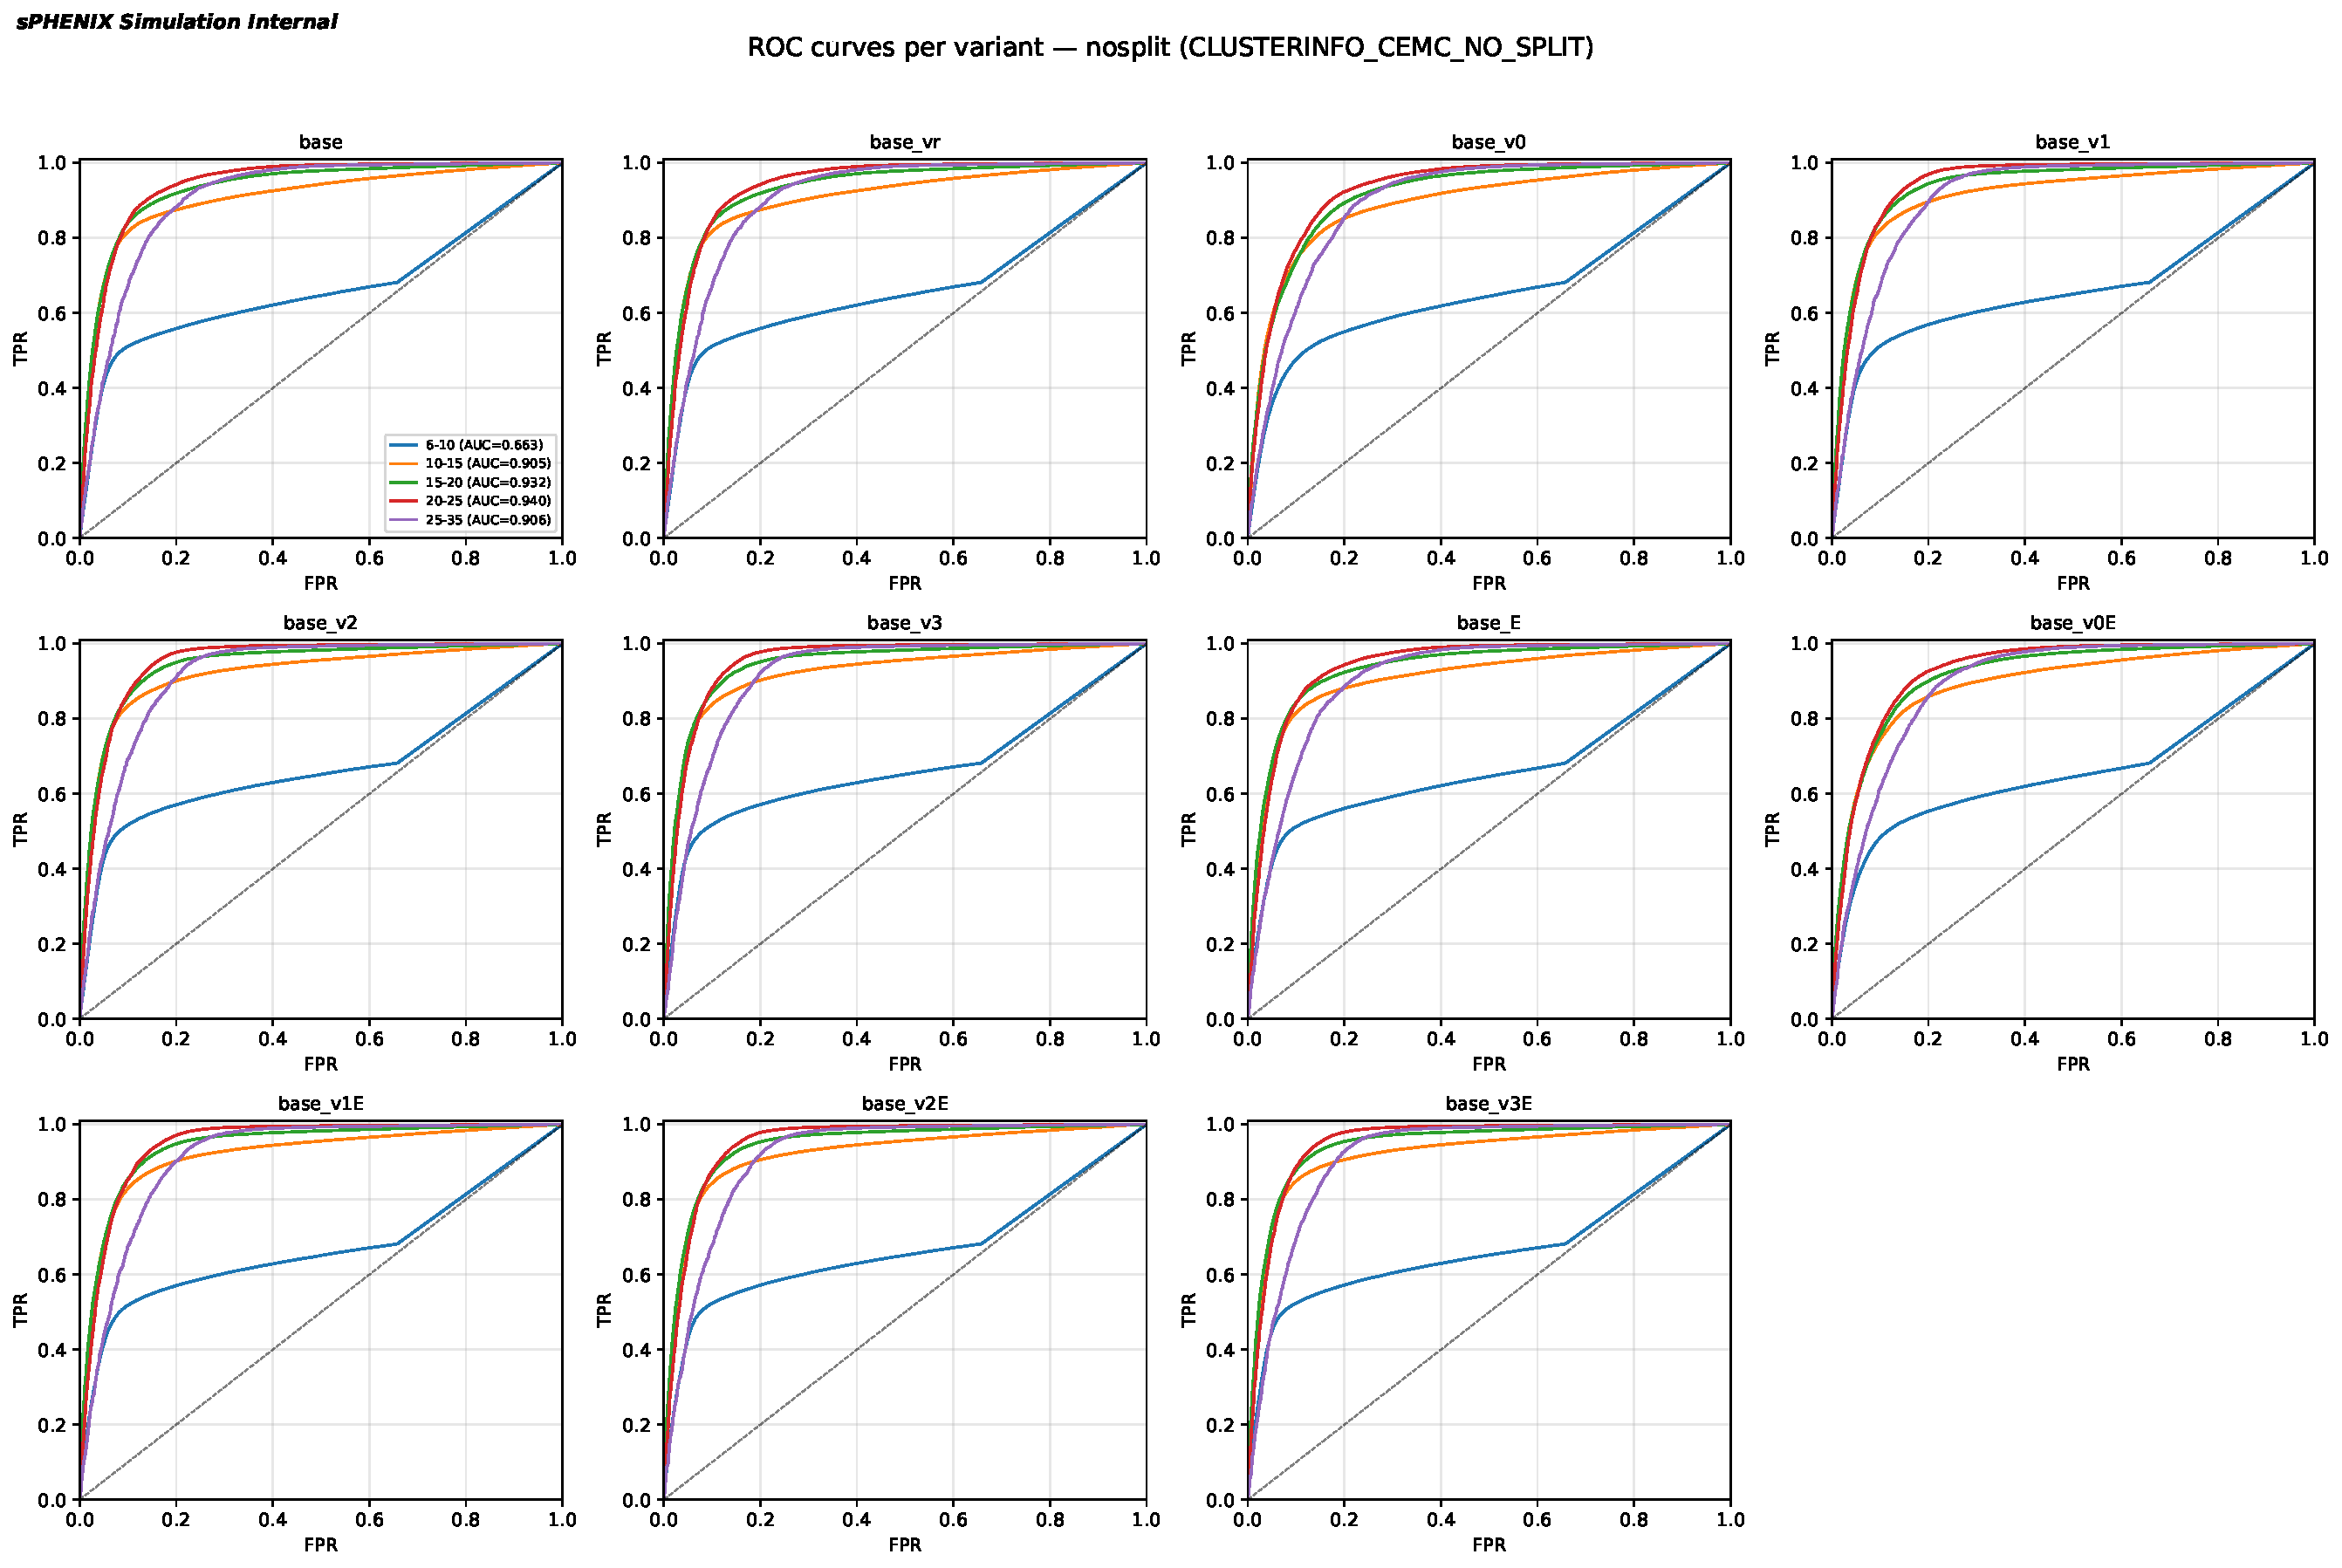
\includegraphics[width=\textwidth]{figures/bdt_audit/roc_grid_nosplit.pdf}
    \caption{As Figure~\ref{fig:bdt_roc_split} but for the nosplit cluster
      node.  AUCs are systematically higher than the split case (consistent
      with the $\approx 5$ percentage-point advantage of the nosplit cluster
      node in Table~\ref{tab:bdt_auc}).}
    \label{fig:bdt_roc_nosplit}
\end{figure}

The BDT score distributions for signal (photon MC) and background (jet MC)
are shown in Figures~\ref{fig:bdt_score_split} and~\ref{fig:bdt_score_nosplit}
for all 11 variants, in the representative $15 < \ET < 20$~\GeV bin.
Background clusters peak sharply near zero in all variants with the expected
shower-shape discrimination; signal photons accumulate at high scores
$> 0.7$.  The \texttt{base\_v0} and \texttt{base\_v0E} panels show much
broader signal distributions extending down to BDT~$\approx 0.3$, reflecting
the weaker discrimination power of dropping $e_{t1}$.  \texttt{base\_vr} is
once again identical to \texttt{base}.

\begin{figure}[H]
    \centering
    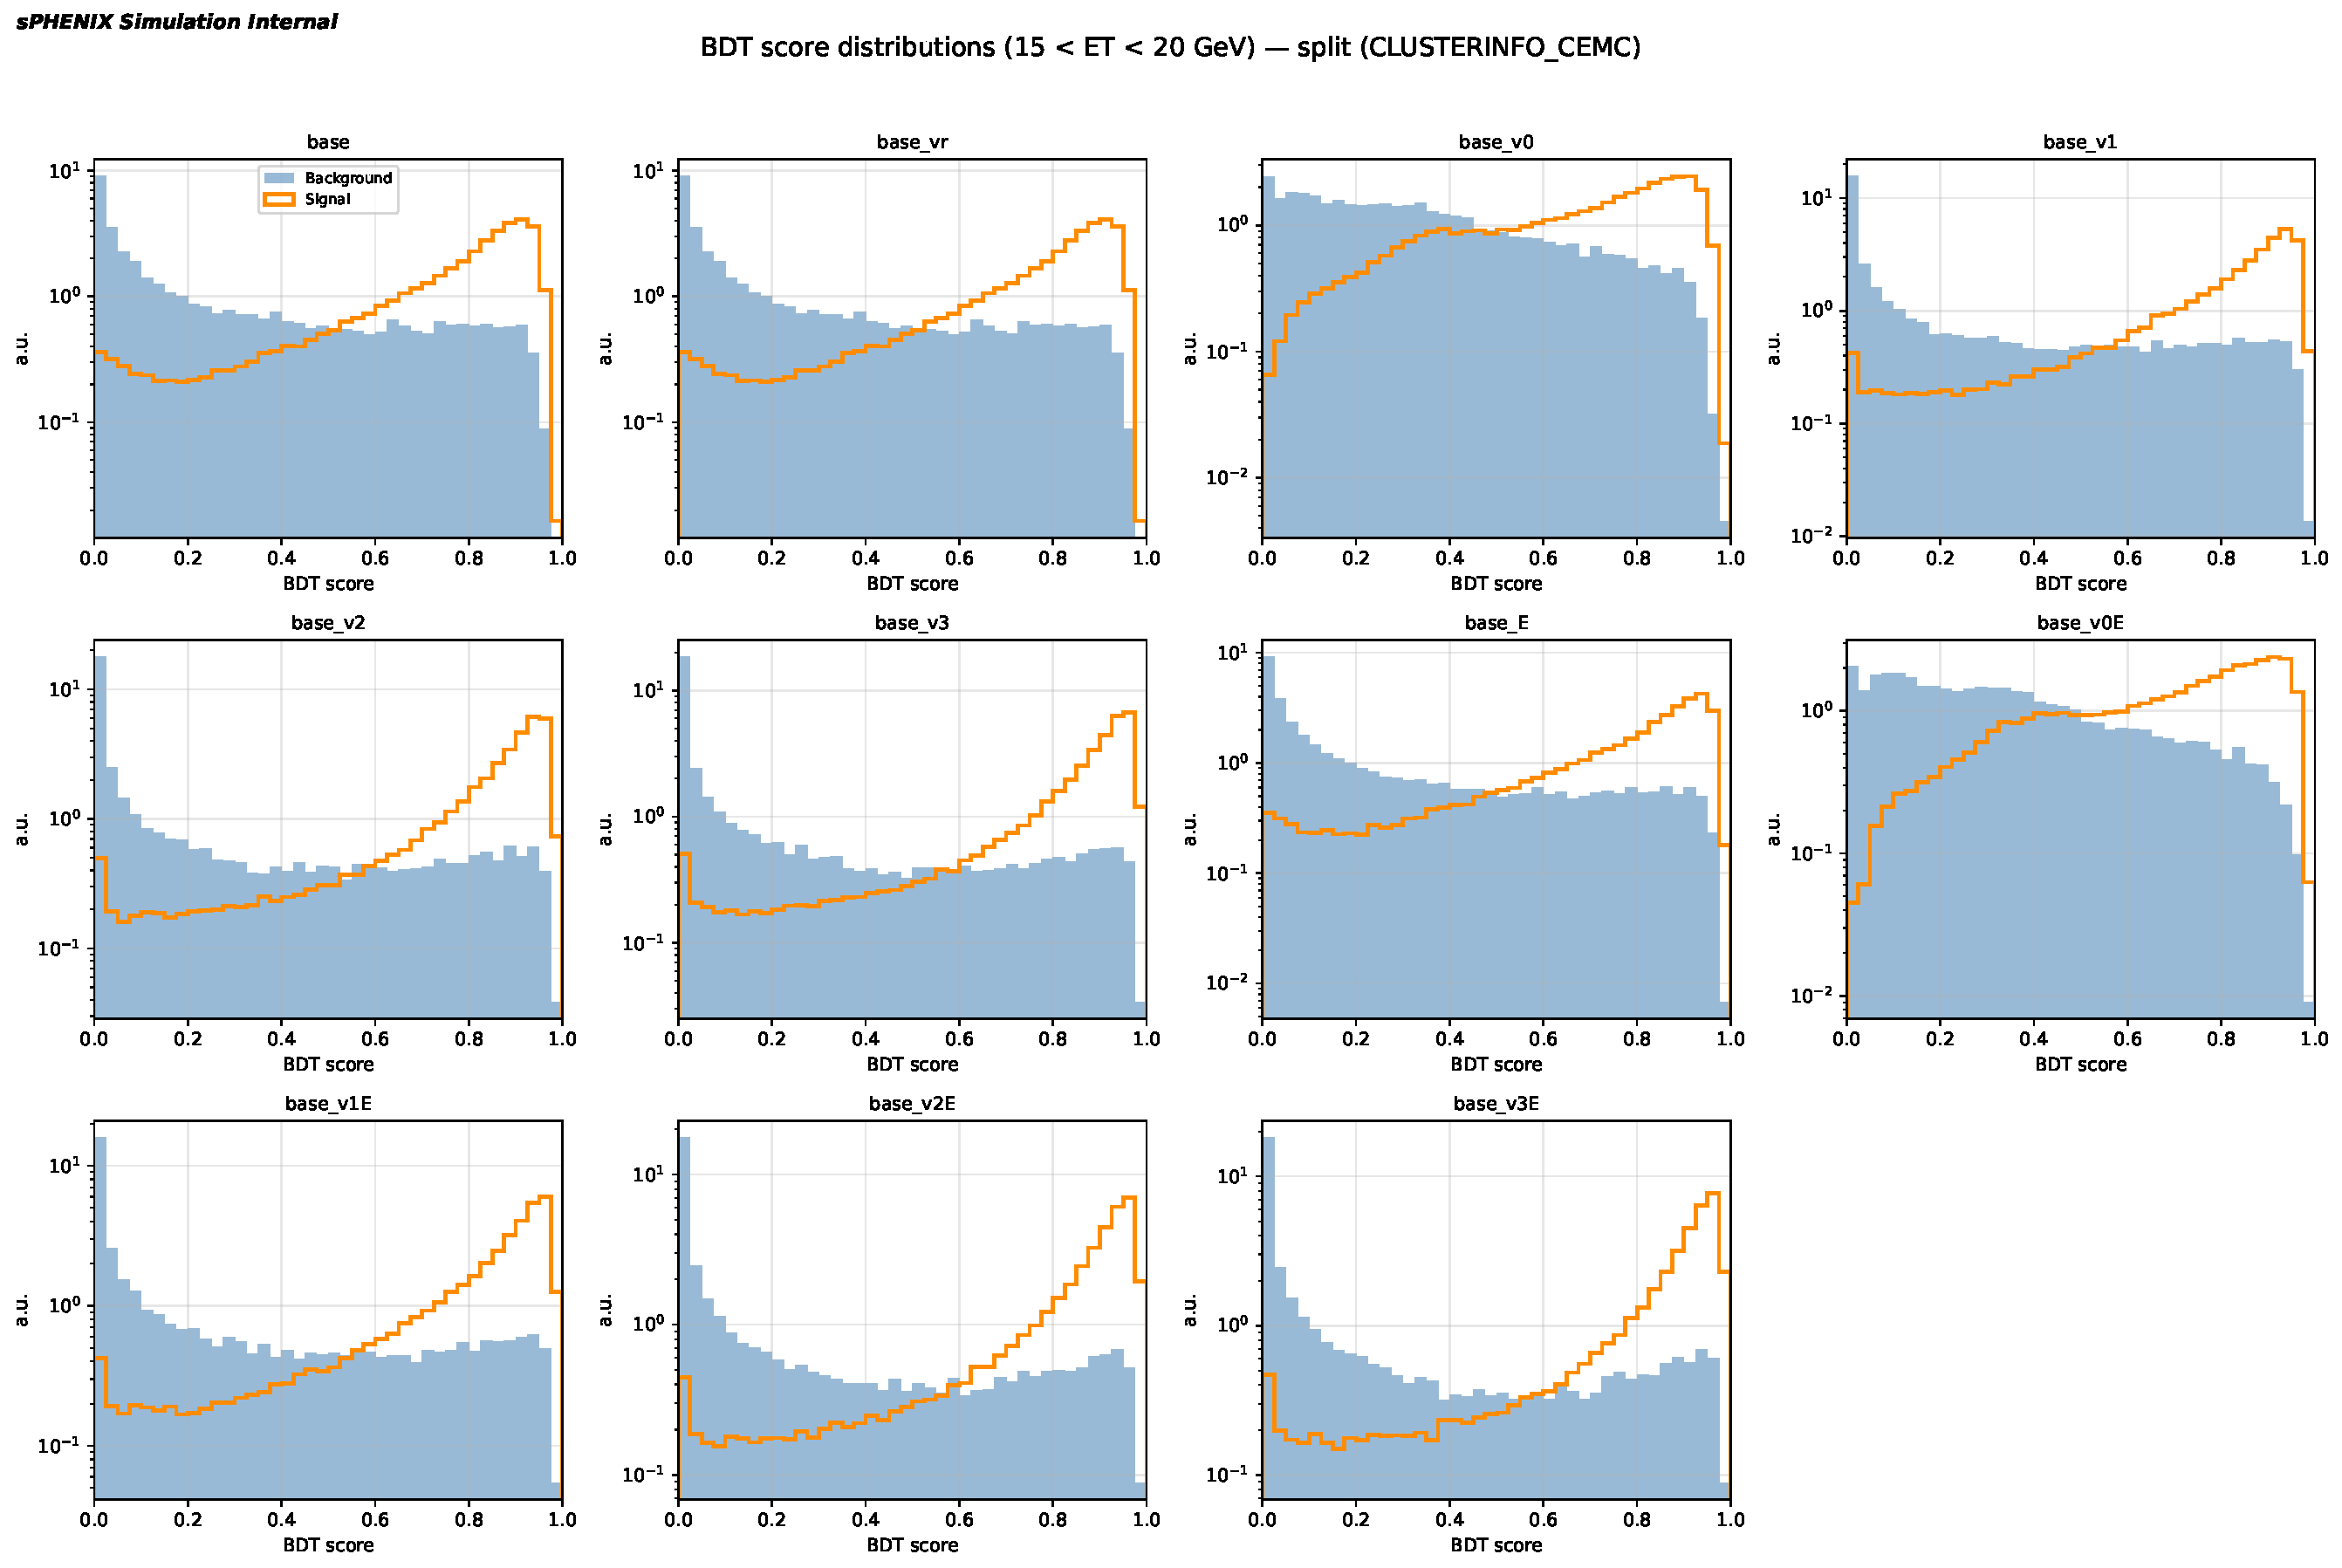
\includegraphics[width=\textwidth]{figures/bdt_audit/bdt_score_grid_split.pdf}
    \caption{BDT score distributions for signal (orange outline) and
      background (blue filled) in the $15 < \ET < 20$~\GeV bin, for all 11
      variants on the split cluster node.  Histograms are unit-normalized;
      log scale on the vertical axis.}
    \label{fig:bdt_score_split}
\end{figure}

\begin{figure}[H]
    \centering
    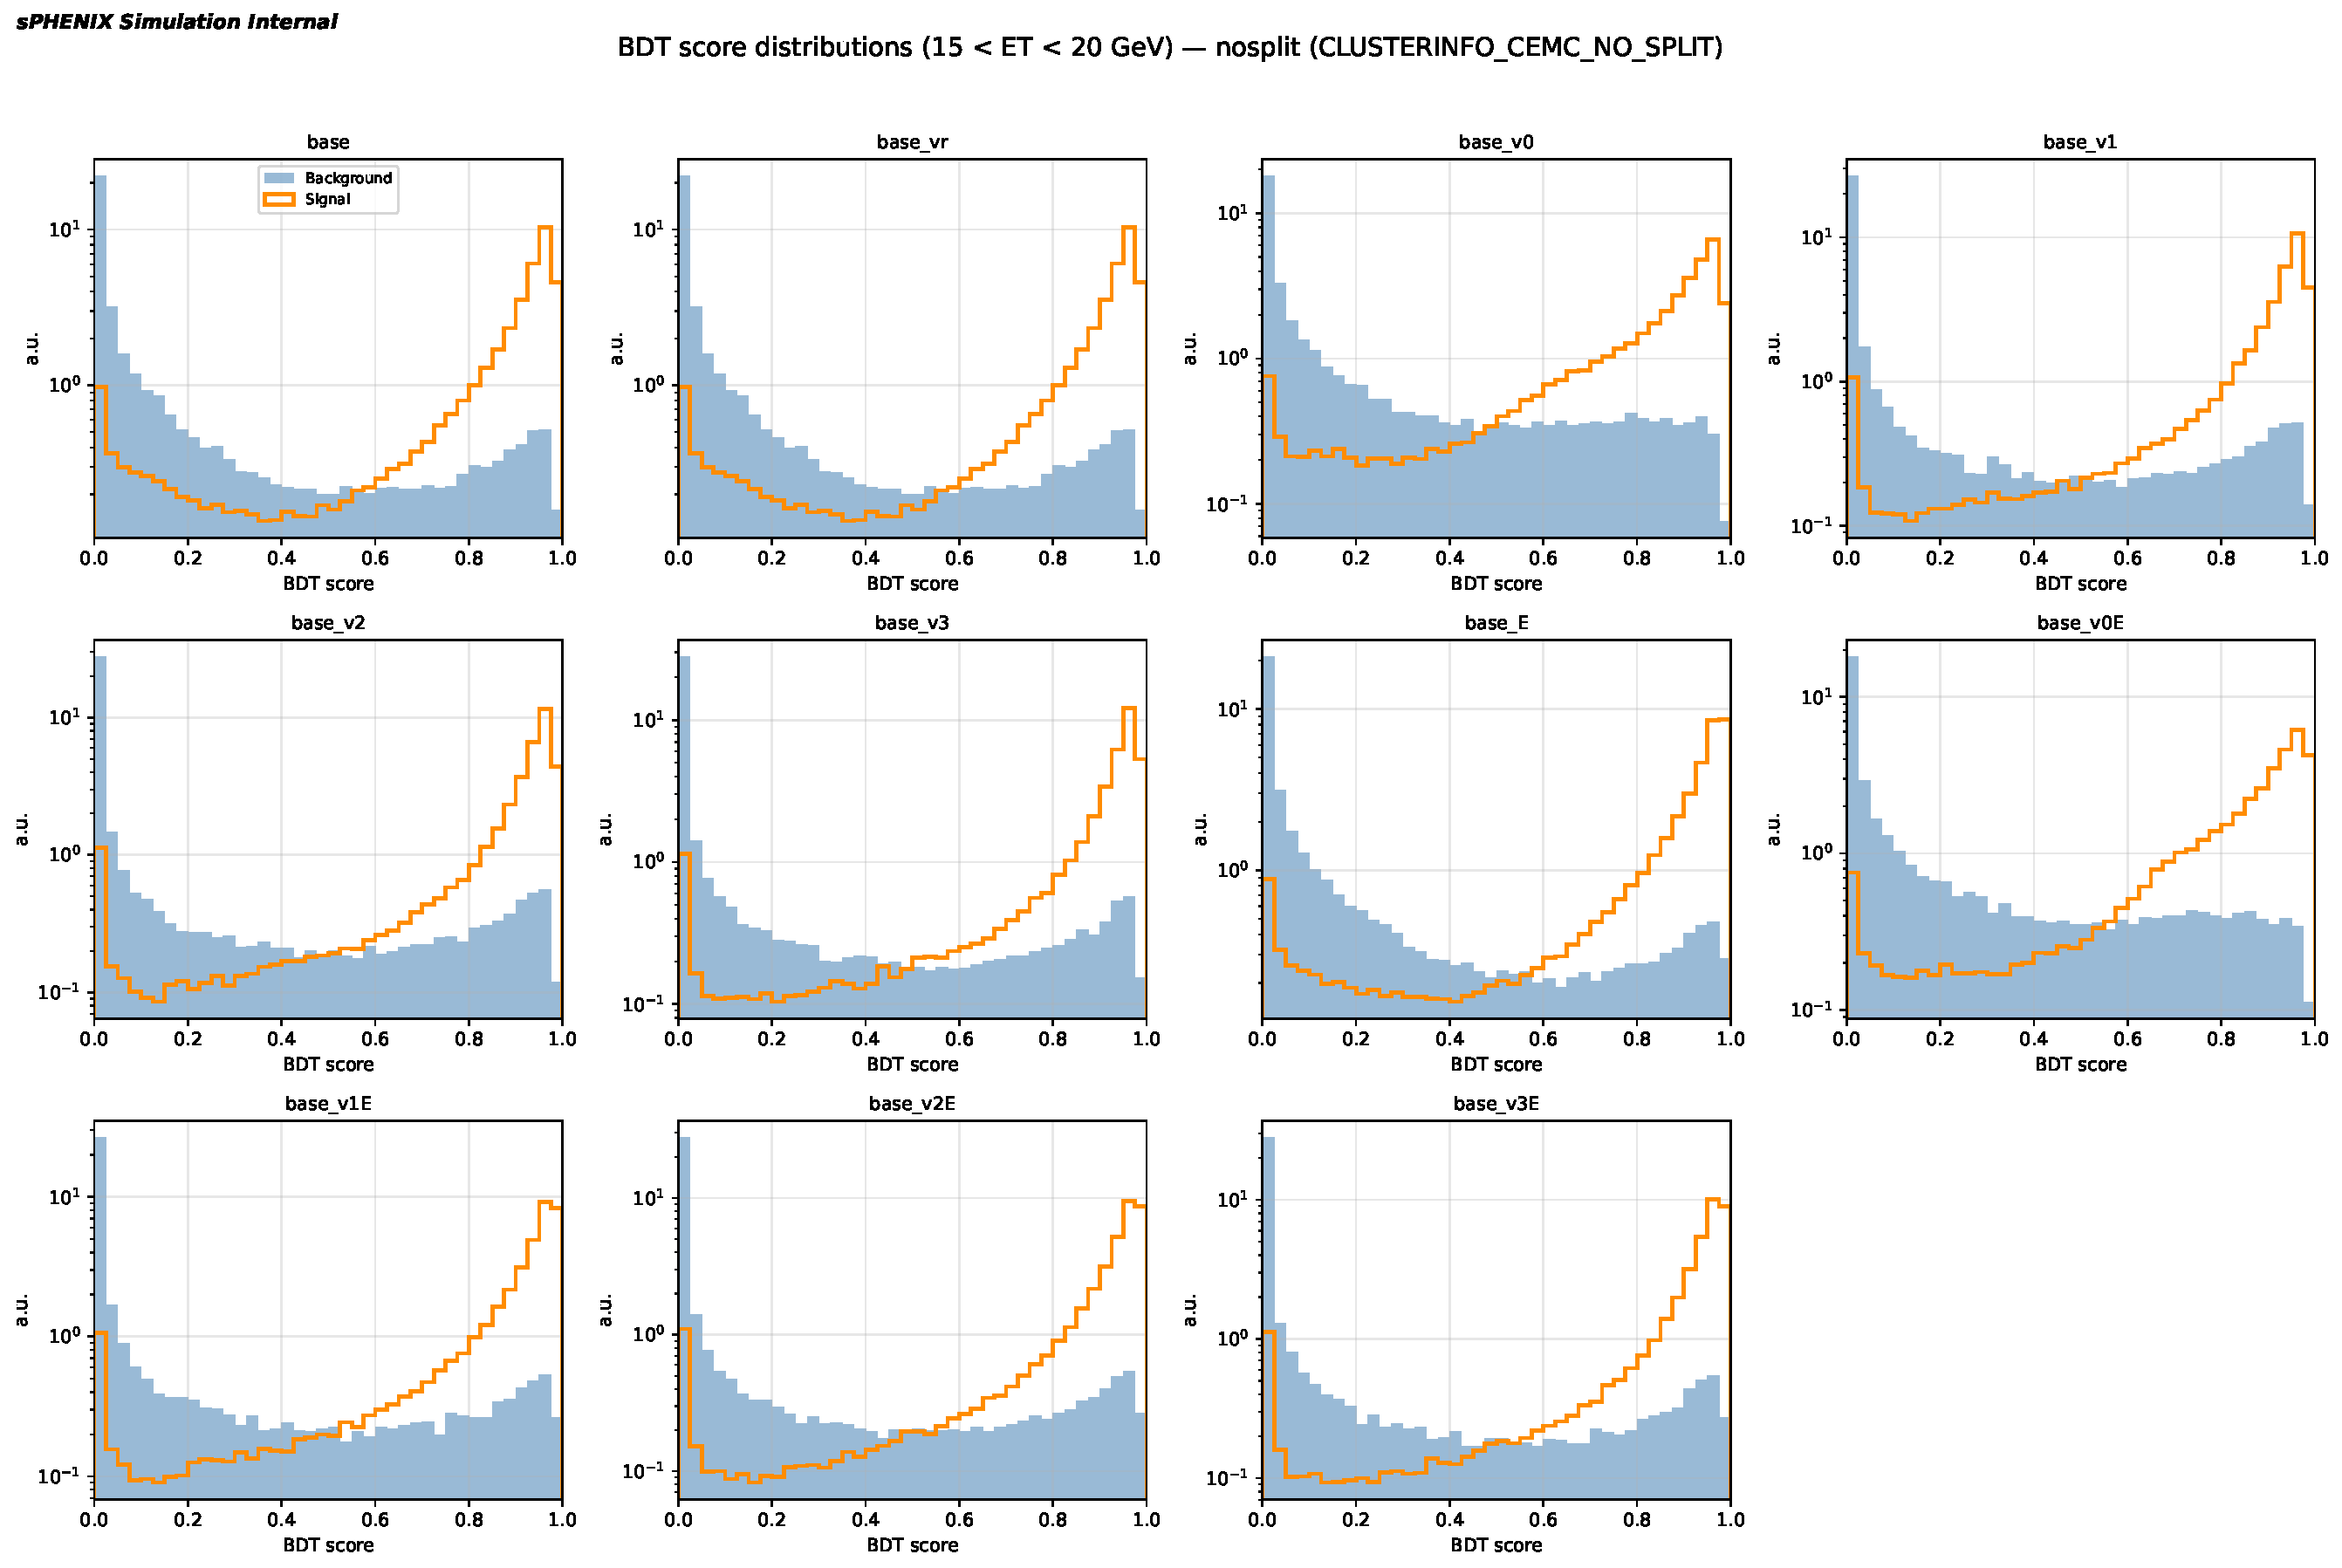
\includegraphics[width=\textwidth]{figures/bdt_audit/bdt_score_grid_nosplit.pdf}
    \caption{As Figure~\ref{fig:bdt_score_split} but for the nosplit cluster
      node.}
    \label{fig:bdt_score_nosplit}
\end{figure}

Figure~\ref{fig:bdt_importance} shows the XGBoost feature importance
(gain metric) for the nine input features of \texttt{base\_v1E}, broken
down by \ET bin.  The tower energy fraction $e_{t1}$ dominates the gain,
contributing 36\% of the total split improvement.  The quadrant
asymmetries ($e_{t2}$, $e_{t3}$), vertex $z$, and $w_\eta^{\text{CoG}}$
provide the next tier of discrimination, while $E_{1\times1}/E_{3\times3}$
and cluster $\eta$ contribute at the 5\% level.  The stability of the
ranking across \ET bins confirms that the model does not rely on
\ET-dependent shortcuts.

\begin{figure}[H]
    \centering
    \includegraphics[width=\textwidth]{../FunWithxgboost/binned_models/model_base_v1E_feature_importance_comparison.pdf}
    \caption{Feature importance for the nominal \texttt{base\_v1E} model,
      shown as gain (left), weight (center), and cover (right) across
      the five \ET training bins.  The tower fraction $e_{t1}$ provides the
      largest gain contribution in all bins.}
    \label{fig:bdt_importance}
\end{figure}

An important consideration for the ABCD background subtraction is the
correlation between the BDT score (defining the tight/non-tight axis) and
the isolation energy \isoET (defining the isolated/non-isolated axis).
Figure~\ref{fig:bdt_isoet} shows the 2D scatter of \isoET vs.\ BDT score
for signal and background clusters.  The overall Spearman correlation
coefficient is $\rho = -0.585$, driven primarily by the background
population where non-isolated jets naturally receive low BDT scores.
The signal photons cluster in the upper-left corner (high BDT, low
\isoET), well separated from the background.  The residual correlation
is accounted for in the ABCD method through the signal leakage
corrections $c_B$, $c_C$, and $c_D$.

\begin{figure}[H]
    \centering
    \includegraphics[width=0.6\textwidth]{../FunWithxgboost/binned_models/model_base_v1E_isoet_bdt_correlation_global.pdf}
    \caption{Scatter plot of reconstruction-level isolation energy \isoET
      vs.\ BDT score for signal (blue) and background (red) clusters,
      nominal \texttt{base\_v1E} model.
      The overall Spearman correlation is $\rho = -0.585$.  Signal photons
      are concentrated at high BDT score and low \isoET, while background
      jets populate the low-score, high-\isoET region.}
    \label{fig:bdt_isoet}
\end{figure}

To make the iso\,vs.\,BDT behaviour easier to read across models, the same
distribution is re-plotted with the axes swapped (BDT score on the
horizontal axis, \isoET on the vertical) and a binned profile of the
mean \isoET per BDT-score bin overlaid for signal and background
separately.  Figures~\ref{fig:bdt_isoet_profile_split}
and~\ref{fig:bdt_isoet_profile_nosplit} show this profile view for all
11 photon-ID variants on the \texttt{CLUSTERINFO\_CEMC} (split) and
\texttt{CLUSTERINFO\_CEMC\_NO\_SPLIT} (nosplit) cluster nodes
respectively.  In every panel the signal profile drops from
$\approx 5$~\GeV at the low-BDT tail to $\lesssim 2$~\GeV above
BDT~$\approx 0.6$, while the background profile stays near
$\sim 10$~\GeV with only a shallow slope --- confirming that the BDT
defines an essentially ABCD-usable axis for all variants, with the
residual correlation absorbed into the signal-leakage corrections
$c_B, c_C, c_D$.  The \texttt{base\_vr} panel is bit-identical to
\texttt{base} across both cluster nodes, re-confirming that the
``vertex reweight'' variant is currently dead (the
\texttt{reweighting.vertex\_reweight: true} override is never injected
into the generated variant configs --- see the BDT training audit note
for details).

\begin{figure}[H]
    \centering
    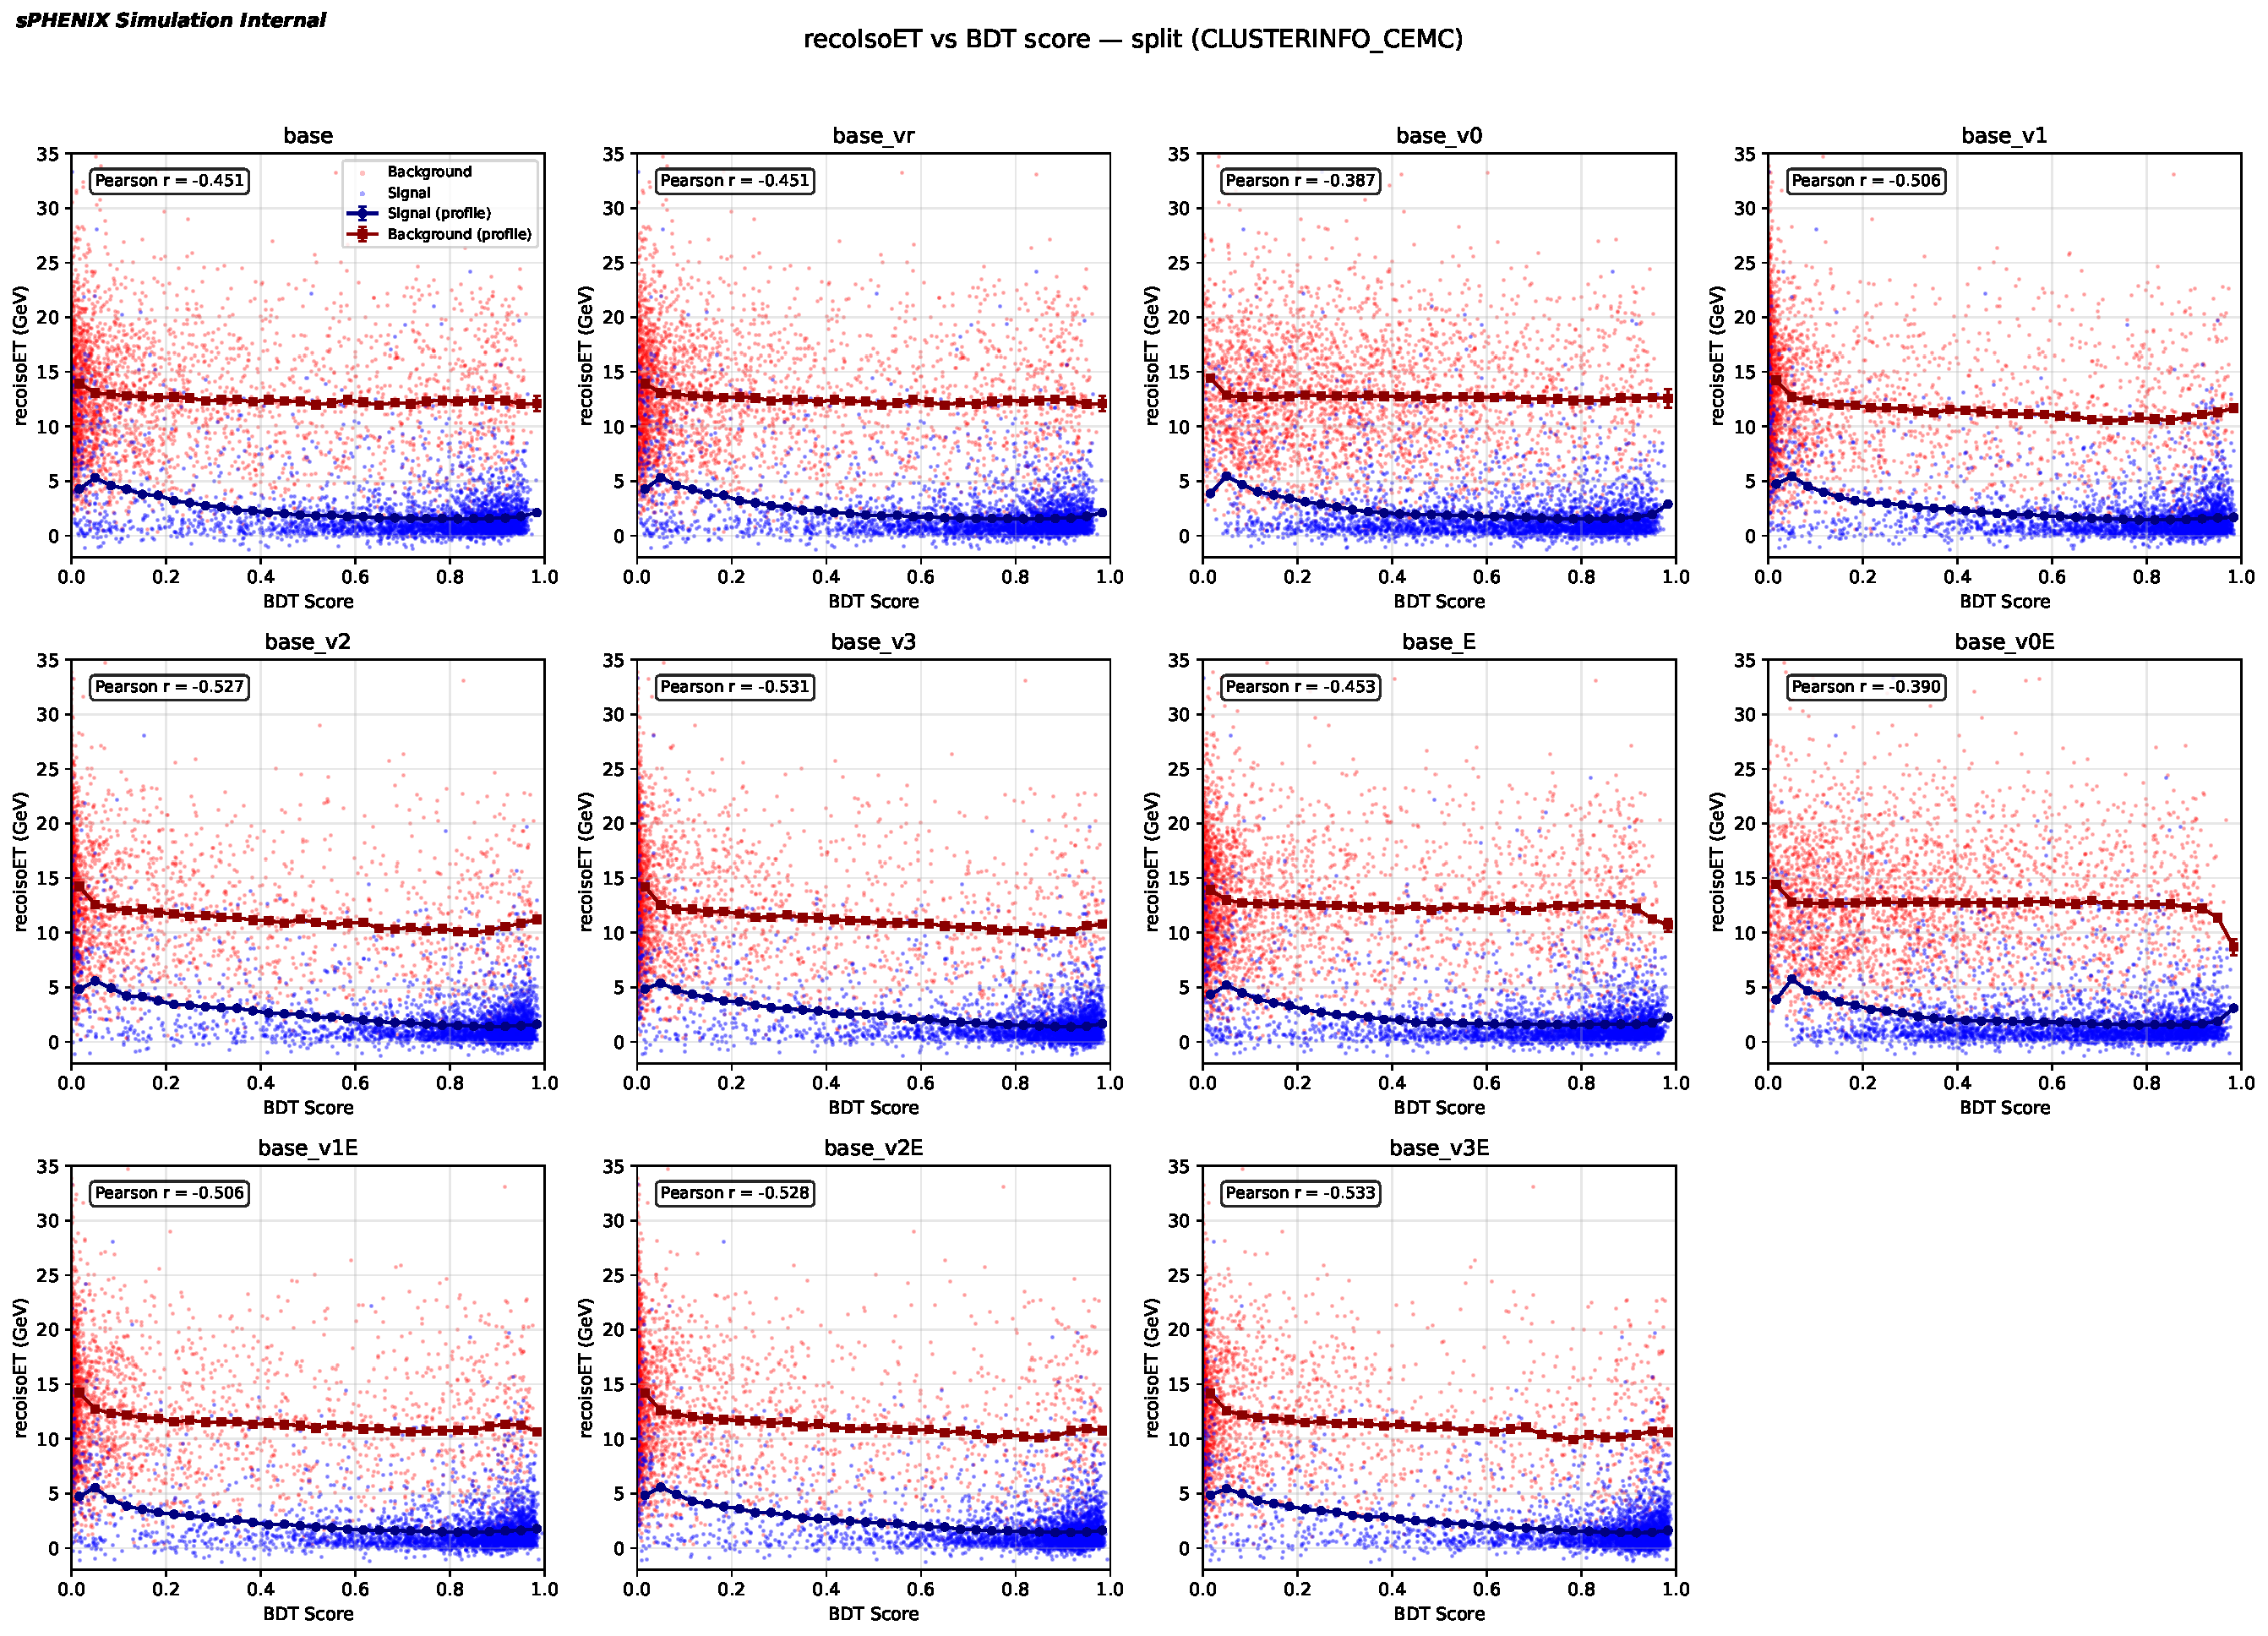
\includegraphics[width=\textwidth]{figures/bdt_audit/profile_isoET_vs_BDT_grid_split.pdf}
    \caption{\isoET\ vs.\ BDT score profile for all 11 photon-ID variants
      on the split cluster node (\texttt{CLUSTERINFO\_CEMC}).  In each
      panel, 4000 random clusters per class are scatter-plotted (signal
      blue, background red); connected markers show the binned profile
      mean $\pm$ SEM of \isoET\ per BDT-score bin (navy: signal, dark
      red: background).  The overall Pearson $r$ (combined pool) is
      quoted in each panel.  Statistics: $\sim 380$\,k signal and
      $\sim 210$\,k background clusters from
      \texttt{photon5/10/20} and \texttt{jet20/30} MC after
      $6<\ET<40$~\GeV, $|\eta|<0.7$.}
    \label{fig:bdt_isoet_profile_split}
\end{figure}

\begin{figure}[H]
    \centering
    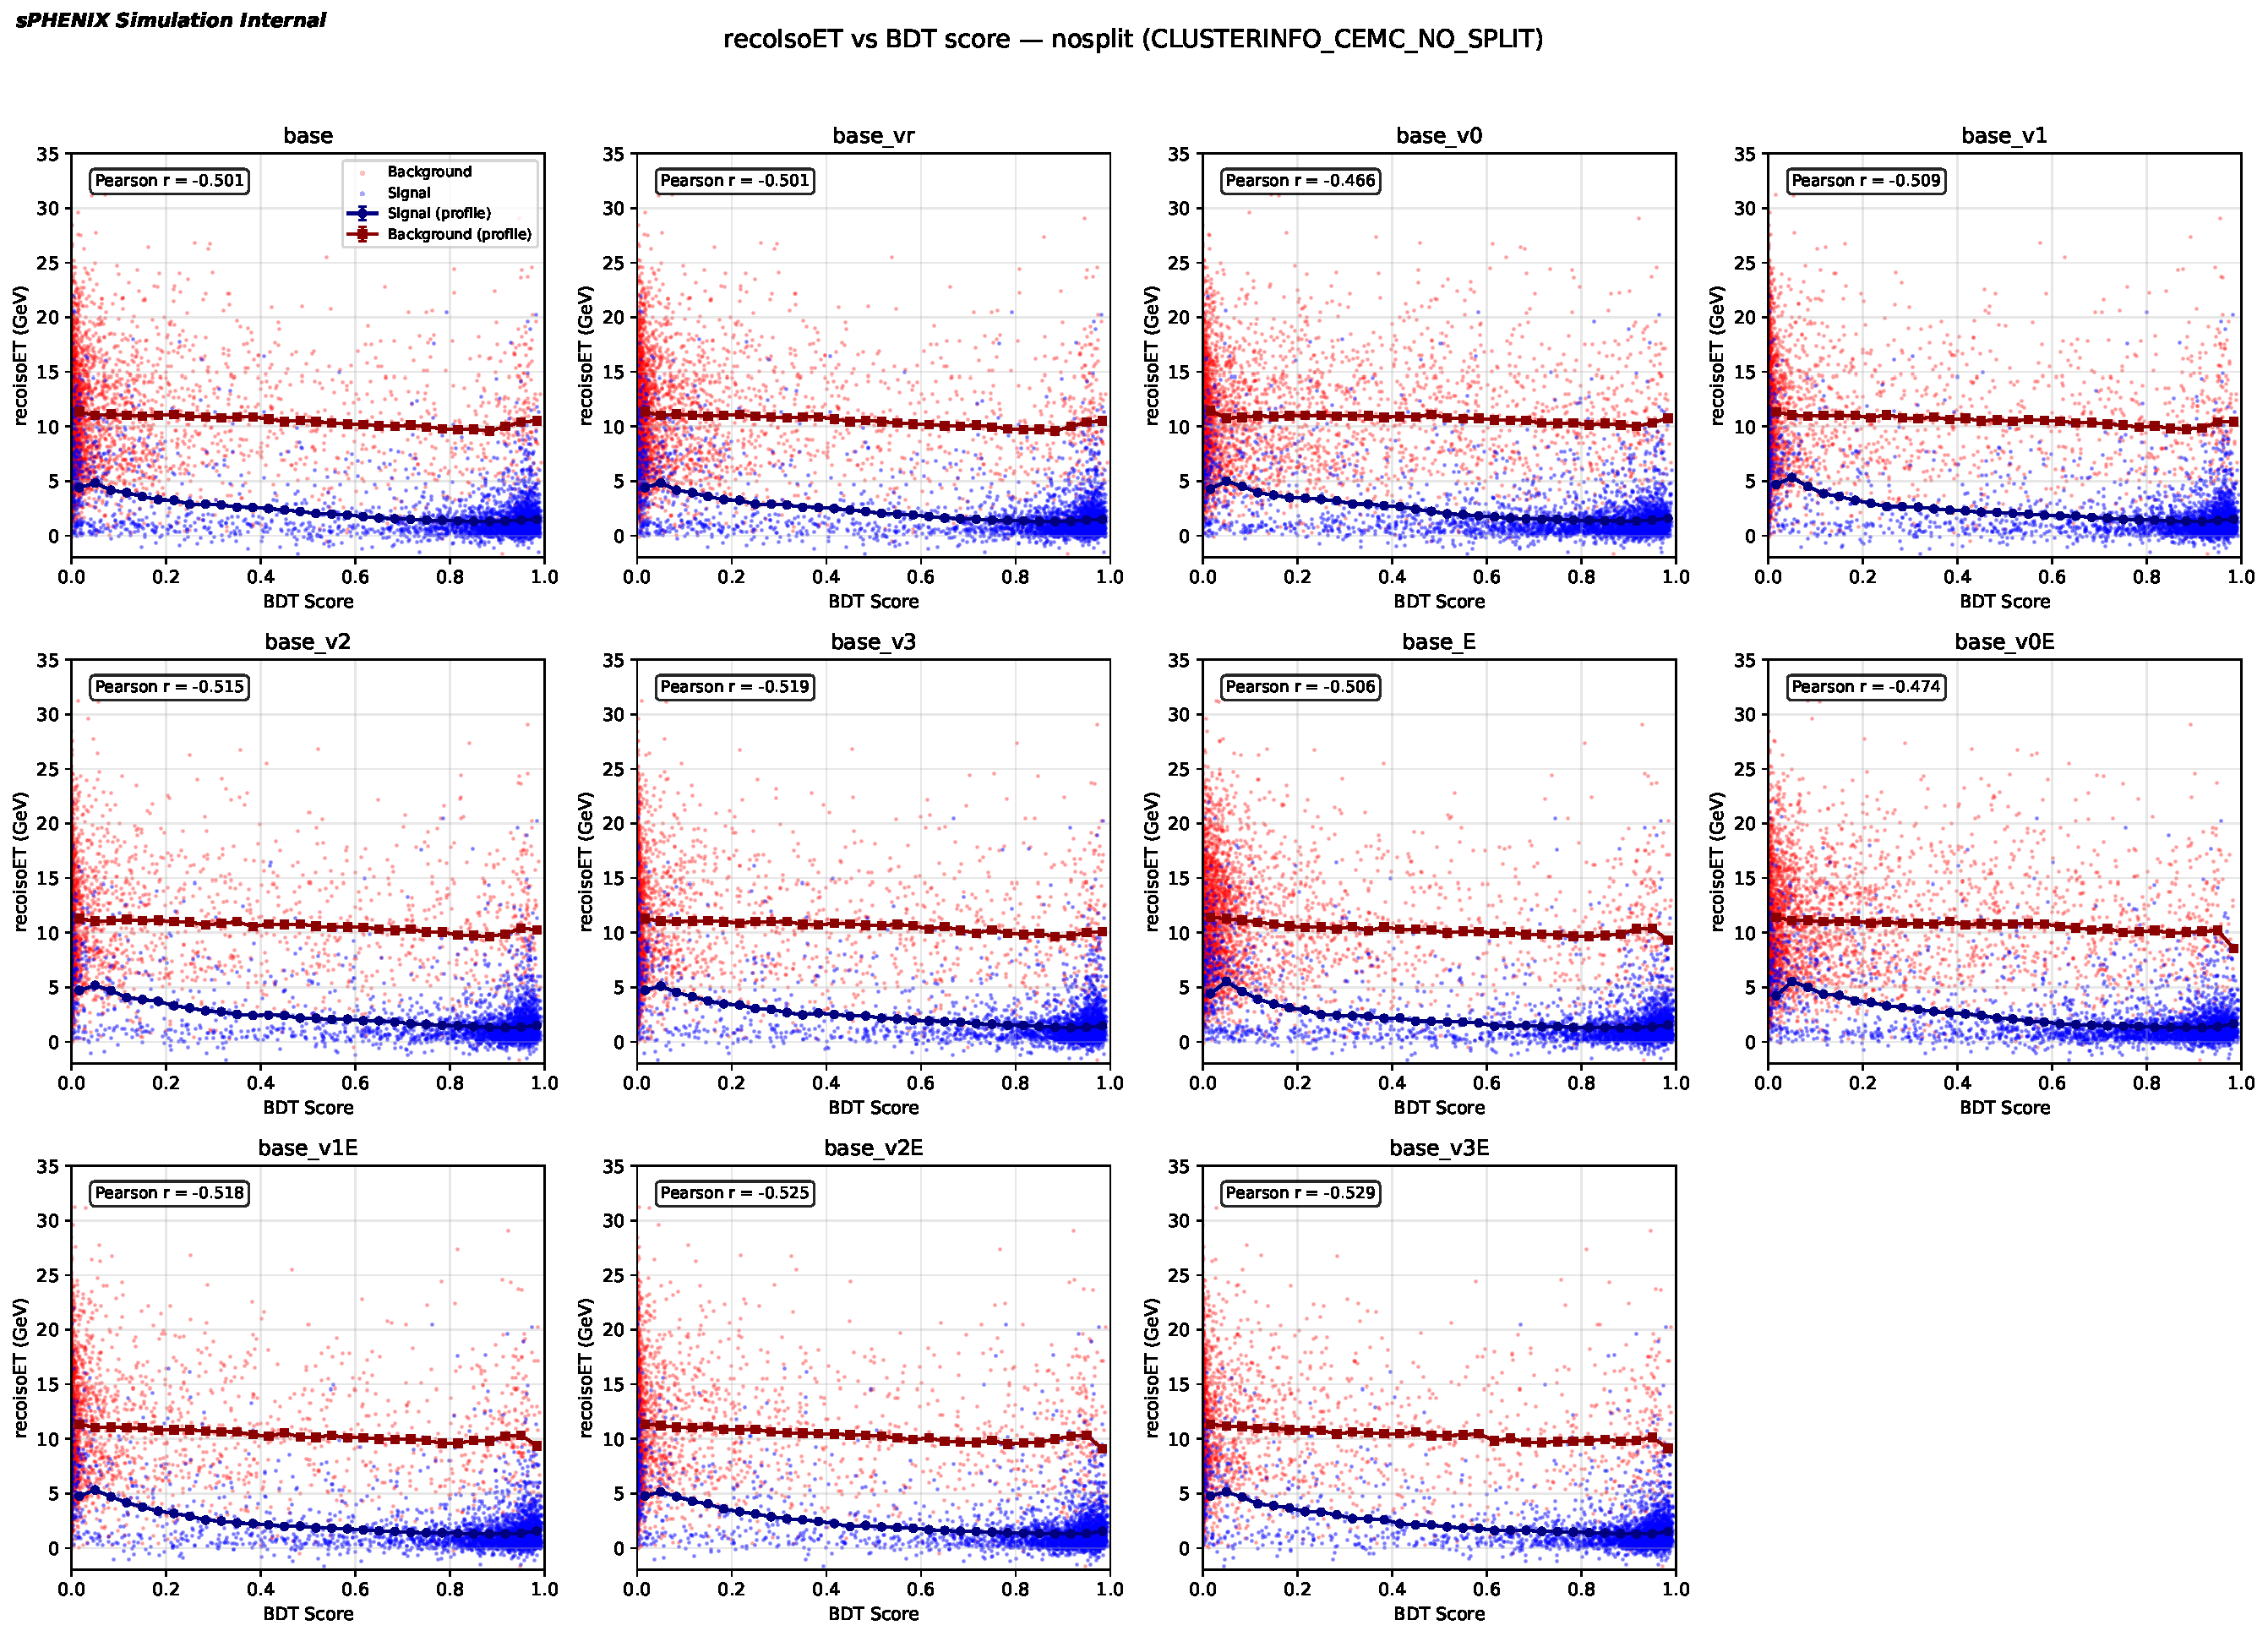
\includegraphics[width=\textwidth]{figures/bdt_audit/profile_isoET_vs_BDT_grid_nosplit.pdf}
    \caption{As Figure~\ref{fig:bdt_isoet_profile_split} but for the
      nosplit cluster node (\texttt{CLUSTERINFO\_CEMC\_NO\_SPLIT}).  The
      signal profile drops more steeply with BDT score and the
      background profile sits slightly lower than in the split case,
      consistent with the $\sim 5$ percentage-point higher test AUCs of
      the nosplit models.}
    \label{fig:bdt_isoet_profile_nosplit}
\end{figure}

\subsection{\ET-Dependent Parametric Threshold}
\label{subsec:bdt_threshold}

The preliminary analysis used a flat BDT threshold. The updated analysis
implements an \ET-dependent parametric cut:
\begin{equation}
    \text{BDT}_{\min}^{\text{tight}} = 0.80 - 0.015 \times \ET\,[\GeV],
    \label{eq:bdt_threshold}
\end{equation}
where the intercept and slope are configurable in the analysis YAML.
This accommodates the improving signal-to-background ratio at higher \ET,
allowing a looser BDT requirement where the background contamination is
naturally lower.

Clusters with $\ET < 7$~\GeV receive a default BDT score of $-1$ and are
excluded from the analysis.

\subsection{BDT Systematic Variations}
\label{subsec:bdt_syst}

The systematic uncertainty framework for the BDT is implemented through
automated config generation (\texttt{make\_bdt\_variations.py}), producing 30+
analysis configurations.  Key BDT-related variations:

\begin{table}[H]
    \centering
    \caption{BDT-related systematic variations. Each variation generates a
      separate analysis config with a unique \texttt{var\_type} suffix.}
    \label{tab:bdt_syst}
    \begin{tabular}{llll}
        \toprule
        Variation & Parameter change & Syst.\ type & Role \\
        \midrule
        \texttt{tightbdt50} & Intercept $\to 0.70$ & Efficiency & Down \\
        \texttt{tightbdt70} & Intercept $\to 0.90$ & Efficiency & Up \\
        \texttt{ntbdtmin05} & Non-tight lower $\to 0.05$ & Purity & One-sided \\
        \texttt{ntbdtmin10} & Non-tight lower $\to 0.10$ & Purity & One-sided \\
        \texttt{etbin\_v3E\_v3E} & Both bins use \texttt{base\_v3E} & Efficiency & Max-envelope \\
        \texttt{etbin\_E\_E} & Both bins use \texttt{base\_E} & Efficiency & Max-envelope \\
        \texttt{etbin\_v1E\_v3E} & Mixed models & Efficiency & Max-envelope \\
        \bottomrule
    \end{tabular}
\end{table}

The tight BDT threshold variation yields 5--10\% relative systematic
uncertainty on the cross-section. The non-tight lower boundary variation
contributes up to 15\% relative uncertainty, primarily affecting the purity
estimate through the ABCD sideband definition.


%% =================================================================
\section{Non-Physics Background Rejection}
\label{sec:npb}

\subsection{From Hard Cut to BDT Score}
\label{subsec:npb_transition}

The preliminary analysis rejected non-physics background (NPB) clusters using a
hard timing preselection: clusters with $t_{\text{cluster}} - t_{\text{MBD}} < -5$~ns
were tagged as NPB and removed.
This approach has two limitations: (1)~the timing threshold is somewhat arbitrary,
and (2)~it provides no discrimination for NPB clusters that happen to arrive
near $t = 0$.

The updated analysis replaces this with a dedicated 25-feature XGBoost model
that scores each cluster on a continuous $[0, 1]$ scale, where high scores
indicate physics clusters and low scores indicate NPB.

\subsection{NPB Score Training}
\label{subsec:npb_training}

The NPB BDT is trained on:
\begin{itemize}
    \item \textbf{Signal (physics)}: Clusters from \textsc{pythia} jet MC
      (jet10, jet15, jet20, jet30, jet50) with valid particle ID,
      $6 < \ET < 40$~\GeV, $|\eta| < 0.7$.
    \item \textbf{Background (NPB)}: Clusters from collision data with
      $t_{\text{cluster}} - t_{\text{MBD}} < -7$~ns, which are
      overwhelmingly beam-induced backgrounds not synchronized with
      the collision time.
\end{itemize}

The model uses 25 input features: cluster \ET, $\eta$, vertex $z$, ten tower
energy ratios ($E_{1\times1}/E_{3\times3}$, $E_{3\times2}/E_{3\times5}$,
$E_{1\times1}/E_{2\times2}$, $E_{1\times1}/E_{1\times3}$, etc.), cluster width
moments ($w_\eta^{\text{CoG}}$, $w_\phi^{\text{CoG}}$, $w_{3\times2}$,
$w_{5\times2}$, $w_{7\times2}$), and tower energy fractions ($e_{t1}$--$e_{t4}$).

\begin{table}[H]
    \centering
    \caption{XGBoost hyperparameters for the NPB score model. Note the differences
      from the photon ID BDT (Table~\ref{tab:xgb_params}): deeper trees and less
      aggressive regularization, reflecting the cleaner signal--background separation
      for NPB rejection.}
    \label{tab:npb_params}
    \begin{tabular}{lc}
        \toprule
        Parameter & Value \\
        \midrule
        Number of boosted trees & 750 \\
        Maximum depth & 6 \\
        Learning rate & 0.1 \\
        Subsample fraction & 0.8 \\
        Column sample per tree & 0.8 \\
        L1 regularization ($\alpha$) & 1.0 \\
        L2 regularization ($\lambda$) & 1.0 \\
        \bottomrule
    \end{tabular}
\end{table}

The trained model is exported to ROOT TMVA format and applied in
\texttt{apply\_BDT.C}, producing a new branch
\texttt{cluster\_npb\_score\_CLUSTERINFO\_CEMC} for each cluster with
$6 < \ET < 40$~\GeV and $|\eta| < 0.7$.

\subsection{NPB Score Validation}
\label{subsec:npb_validation}

The NPB score is validated independently using the cluster--MBD timing
distribution $t_{\text{cluster}} - t_{\text{MBD}}$:
\begin{itemize}
    \item At NPB score $> 0.5$: the timing distribution is sharply peaked near
      $t = 0$~ns, confirming physics origin.
    \item At NPB score $< 0.2$: the distribution is broad, extending to large
      negative times ($t < -7$~ns), confirming NPB origin.
\end{itemize}
A background template is constructed from the out-of-time tail ($t < -7$~ns) and
normalized to estimate the NPB fraction as a function of the score threshold.

Figure~\ref{fig:npb_bkg_timing} shows the cluster--MBD time distributions in
data for three representative \ET bins, with the low-NPB-score background
template overlaid.
The template (normalized in the $t < -7$~ns tail) matches the out-of-time
component, demonstrating that the NPB score correctly identifies beam-background
clusters independently of the timing variable used to define the training labels.

\begin{figure}[H]
    \centering
    \begin{subfigure}[t]{0.48\textwidth}
        \includegraphics[width=\textwidth]{../PPG12-analysis-note/Figures/npb_time_bkgsub/npb_time_bkg_overlay_eta0_pt0.pdf}
        \caption{$10 < \ET < 14$~\GeV}
    \end{subfigure}
    \hfill
    \begin{subfigure}[t]{0.48\textwidth}
        \includegraphics[width=\textwidth]{../PPG12-analysis-note/Figures/npb_time_bkgsub/npb_time_bkg_overlay_eta0_pt1.pdf}
        \caption{$14 < \ET < 18$~\GeV}
    \end{subfigure}
    \\[6pt]
    \begin{subfigure}[t]{0.48\textwidth}
        \includegraphics[width=\textwidth]{../PPG12-analysis-note/Figures/npb_time_bkgsub/npb_time_bkg_overlay_eta0_pt2.pdf}
        \caption{$18 < \ET < 22$~\GeV}
    \end{subfigure}
    \hfill
    \begin{subfigure}[t]{0.48\textwidth}
        \includegraphics[width=\textwidth]{../PPG12-analysis-note/Figures/npb_time_bkgsub/npb_time_bkg_overlay_eta0_pt3.pdf}
        \caption{$22 < \ET < 28$~\GeV}
    \end{subfigure}
    \caption{Cluster--MBD time distributions in data (black) with low-NPB-score
      background template (red, normalized in $t < -7$~ns tail) for four \ET bins.
      The background template tracks the out-of-time tail, confirming the NPB
      score identifies beam backgrounds independent of timing.}
    \label{fig:npb_bkg_timing}
\end{figure}

\subsection{Cut Optimization}
\label{subsec:npb_optimization}

The nominal threshold is set at NPB score $> 0.5$, achieving:
\begin{itemize}
    \item \textbf{NPB purity}: ${\sim}99\%$ of surviving clusters are physics
      (NPB contamination ${\sim}1$--$2\%$).
    \item \textbf{Signal retention}: ${\sim}98\%$ of MC physics clusters pass
      the threshold.
\end{itemize}

Figure~\ref{fig:npb_purity_yield} shows the NPB purity (fraction of physics
clusters) and cluster yield as a function of the NPB score threshold for three
\ET bins.
The purity rises steeply from ${\sim}96\%$ at threshold 0.1 to ${\sim}99\%$
at the nominal 0.5, with minimal yield loss.
Figure~\ref{fig:npb_eff} shows the corresponding MC selection efficiency.

\begin{figure}[H]
    \centering
    \begin{subfigure}[t]{0.32\textwidth}
        \includegraphics[width=\textwidth]{../PPG12-analysis-note/Figures/npb_time_bkgsub/purity_vs_npb_eta0_pt0.pdf}
        \caption{$10$--$14$~\GeV}
    \end{subfigure}
    \hfill
    \begin{subfigure}[t]{0.32\textwidth}
        \includegraphics[width=\textwidth]{../PPG12-analysis-note/Figures/npb_time_bkgsub/purity_vs_npb_eta0_pt1.pdf}
        \caption{$14$--$18$~\GeV}
    \end{subfigure}
    \hfill
    \begin{subfigure}[t]{0.32\textwidth}
        \includegraphics[width=\textwidth]{../PPG12-analysis-note/Figures/npb_time_bkgsub/purity_vs_npb_eta0_pt2.pdf}
        \caption{$18$--$22$~\GeV}
    \end{subfigure}
    \caption{Physics-cluster purity as a function of NPB score threshold for
      three \ET bins. Purity is estimated via timing-based background subtraction
      ($t < -7$~ns template). The nominal threshold at 0.5 achieves ${\sim}99\%$
      purity across all bins.}
    \label{fig:npb_purity_yield}
\end{figure}

\begin{figure}[H]
    \centering
    \includegraphics[width=0.75\textwidth]{../PPG12-analysis-note/Figures/npb_efficiency_vs_threshold.pdf}
    \caption{Selection efficiency of the NPB score cut on inclusive MC clusters
      as a function of the NPB threshold. At the nominal threshold of 0.5,
      ${\sim}98\%$ of MC physics clusters are retained.}
    \label{fig:npb_eff}
\end{figure}

\subsection{NPB Systematic Variations}
\label{subsec:npb_syst}

The NPB score threshold is varied as a systematic:
\begin{itemize}
    \item \texttt{npb03}: Threshold $\to 0.3$ (looser, higher NPB contamination)
    \item \texttt{npb07}: Threshold $\to 0.7$ (tighter, lower signal retention)
\end{itemize}
The cross-section deviations from the nominal are taken as bin-by-bin systematic
uncertainties.


%% =================================================================
\section{Double-Interaction Efficiency Study}
\label{sec:double_eff}

\subsection{Motivation}
\label{subsec:di_motivation}

When double-interaction MC samples (produced with full GEANT4 simulation of two
overlapping \pp collisions) were passed through the original efficiency pipeline
(which required $\DR < 0.1$ geometric truth-matching on top of the GEANT track~ID),
the reconstruction efficiency dropped dramatically: from ${\sim}91\%$ (single
interaction) to ${\sim}31\%$ (double interaction).
A dedicated investigation demonstrated that this drop was overwhelmingly a
truth--reco matching artifact caused by vertex displacement.
Based on this finding, the $\DR < 0.1$ requirement was removed from the production
efficiency calculation; track~ID matching alone provides the definitive truth
association.
This section documents both the artifact diagnosis and the corrected efficiency
breakdown after \DR removal.

\subsection{Pileup Fraction Calculation}
\label{subsec:pileup_fractions}

The mean number of collisions per bunch crossing is computed from the
Poisson-corrected MBD coincidence rate:
\begin{equation}
    \mu = \frac{\sum_{\text{runs}} N_{\text{MBD,corr}}}{r_B \cdot \sum_{\text{runs}} \Delta t},
\end{equation}
where $r_B = 111 \times 78{,}200 = 8.68 \times 10^{6}$~Hz is the RHIC bunch
crossing rate.
The event-level interaction fractions are:
\begin{equation}
    f_1 = \frac{\mu\, e^{-\mu}}{1 - e^{-\mu}}, \qquad
    f_2 = \frac{(\mu^2/2)\, e^{-\mu}}{1 - e^{-\mu}}, \qquad
    f_{\geq 3} = 1 - f_1 - f_2.
\end{equation}
Fractions are computed per run and luminosity-weighted (not simple-averaged) to
avoid Jensen's inequality bias.
Cluster-weighted fractions account for the higher cluster multiplicity in
multi-interaction events:
\begin{equation}
    w_{\text{single}} = \frac{f_1}{\sum_k k\, f_k}, \qquad
    w_{\text{double}} = \frac{2\, f_2 + 3\, f_{\geq 3}}{\sum_k k\, f_k}.
\end{equation}

\begin{table}[H]
    \centering
    \caption{Luminosity-weighted pileup fractions and cluster-level mixing weights.}
    \label{tab:pileup_fractions}
    \begin{tabular}{lcccccc}
        \toprule
        Crossing angle & Run range & $\mu_{\text{corr}}$ & $f_1$ & $f_2$ & $w_{\text{single}}$ & $w_{\text{double}}$ \\
        \midrule
        0~mrad   & 47289--51274 & 0.24 & 0.879 & 0.111 & 0.776 & 0.224 \\
        1.5~mrad & 51274--54000 & 0.08 & 0.960 & 0.039 & 0.921 & 0.079 \\
        \bottomrule
    \end{tabular}
\end{table}

\subsection{Truth Photon Content}
\label{subsec:truth_content}

A prerequisite for interpreting the efficiency drop is verifying that the
double-interaction MC does not inject additional truth-level prompt photons from
the second collision.

\begin{table}[H]
    \centering
    \caption{Truth-level prompt photon content per event (photon10 samples,
      100k events each). The denominator requires $|\eta^{\gamma}| < 0.7$ and
      $\isoETtruth < 4$~\GeV.}
    \label{tab:truth_content}
    \begin{tabular}{lcc}
        \toprule
        Quantity & Single MC & Double MC \\
        \midrule
        Mean truth photons per event & 0.493 & 0.495 \\
        Events with $\geq 2$ denom.\ photons & 0.22\% & 0.21\% \\
        Mean truth \isoETtruth [\GeV] & 0.17 & 0.26 \\
        \bottomrule
    \end{tabular}
\end{table}

The truth photon content is statistically identical.
The slightly higher mean truth isolation energy in double MC (0.26 vs.\
0.17~\GeV) reflects additional hadrons from the second collision falling within
the isolation cone, but this is well below the 4~\GeV fiducial threshold.

\subsection{Vertex Shift Mechanism}
\label{subsec:vertex_shift}

In double-interaction events, the reconstructed vertex is the average of the two
collision points:
\begin{equation}
    z_{\text{vtx}}^{\text{reco}} = \frac{z_{\text{vtx},1} + z_{\text{vtx},2}}{2}.
\end{equation}
Since both vertices are drawn from a broad distribution (RMS ${\sim}30$~cm), the
displacement $\Delta z = z_{\text{vtx}}^{\text{reco}} - z_{\text{vtx}}^{\text{truth}}$
can be large.
The cluster pseudorapidity shift at EMCal radius $R_{\text{EMCal}} = 93.5$~cm is:
\begin{equation}
    \Delta\eta \approx -\frac{\Delta z}{R_{\text{EMCal}} \cosh\eta},
\end{equation}
which at $\eta = 0$ gives $|\Delta\eta| \approx |\Delta z| / 93.5$~cm.
The $\DR < 0.1$ matching threshold therefore fails when
$|\Delta z| \gtrsim 9.35$~cm at midrapidity.

\begin{table}[H]
    \centering
    \caption{Vertex shift distributions. The critical threshold $|\Delta z| = 9.35$~cm
      corresponds to $|\Delta\eta| = 0.1$ at $\eta = 0$.}
    \label{tab:vertex_shift}
    \begin{tabular}{lcc}
        \toprule
        Quantity & Single MC & Double MC \\
        \midrule
        RMS of $\Delta z$ [cm] & 7.6 & 34.5 \\
        Fraction with $|\Delta z| > 9.35$~cm & --- & 83\% \\
        \bottomrule
    \end{tabular}
\end{table}

The sharp transition in matching failure rate as a function of $|\Delta z|$
confirms the deterministic geometric origin:

\begin{table}[H]
    \centering
    \caption{Matching failure rate vs.\ vertex displacement in double MC.}
    \label{tab:failure_vs_dz}
    \begin{tabular}{lc}
        \toprule
        $|\Delta z|$ range [cm] & Matching failure rate \\
        \midrule
        $< 10$ & 9\% \\
        $10$--$15$ & 77\% \\
        $15$--$20$ & $\sim$100\% \\
        $> 20$ & 100\% \\
        \bottomrule
    \end{tabular}
\end{table}

\subsection{Decomposition of the \DR Matching Failure}
\label{subsec:eff_decomposition}

For truth photons that failed the $\DR < 0.1$ match in double MC, the failure
mode was classified by searching for the \texttt{trkID}-matched cluster
regardless of \DR:

\begin{itemize}
    \item \textbf{\DR failure (88\%)}: A cluster with the correct \texttt{trkID}
      exists but $\DR > 0.1$ due to vertex shift.
      The signal photon cluster is present --- it merely appears at the
      wrong $\eta$ when reconstructed from the displaced vertex.
    \item \textbf{Missing cluster (12\%)}: No cluster with the matching
      \texttt{trkID} is found, corresponding to genuine cluster loss from merging
      in the higher-multiplicity environment.
    \item \textbf{Extra truth photons (${\sim}0\%$)}: The second collision does
      not produce additional prompt photons.
\end{itemize}

This decomposition motivated removing the $\DR < 0.1$ requirement from the
production efficiency calculation.

\subsection{Removal of the \DR Matching Requirement}
\label{subsec:dr_removal}

A dedicated study of single-interaction MC demonstrated that even without pileup,
the $\DR < 0.1$ cut rejects ${\sim}3.5\%$ of correctly \texttt{trkID}-matched
truth photons (Table~\ref{tab:dr_single}).
The rejection is driven entirely by vertex mismatch ($|\Delta z| > 9.35$~cm), not
cluster quality: 73\% of rejected clusters have $\ET / \pT^{\text{truth}} \in
[0.8, 1.2]$.
Six physics arguments support the removal (detailed in the companion report):
the track~ID is ground truth; the cut tests vertex resolution, not calorimeter
performance; the response matrix captures vertex-induced kinematic shifts; and
the ${\sim}3\%$ bias is vertex-dependent.

\begin{table}[H]
    \centering
    \caption{$\DR < 0.1$ failure rates in single-interaction MC. ``Fail \DR''
      is the fraction of \texttt{trkID}-matched photons rejected by the geometric cut.}
    \label{tab:dr_single}
    \begin{tabular}{lccc}
        \toprule
        Sample & Truth photons & No trkID match & Fail $\DR < 0.1$ (of matched) \\
        \midrule
        photon5  & 273{,}017   & 3.42\% & 2.70\% \\
        photon10 & 2{,}380{,}500 & 2.37\% & 2.98\% \\
        photon20 & 2{,}840{,}703 & 1.72\% & 4.01\% \\
        \midrule
        Combined & 5{,}494{,}220 & 2.09\% & 3.50\% \\
        \bottomrule
    \end{tabular}
\end{table}

\begin{figure}[H]
    \centering
    \includegraphics[width=0.75\textwidth]{../plotting/figures/deltaR_study/fail_fraction_vs_dz.pdf}
    \caption{$\DR < 0.1$ failure fraction as a function of $|\Delta z|$ in
      single-interaction MC. The sharp step at ${\sim}9.35$~cm matches the
      geometric prediction from the EMCal barrel radius, confirming vertex
      mismatch as the sole driver of the matching failure.}
    \label{fig:fail_vs_dz}
\end{figure}

\subsection{Per-Component Efficiency Breakdown (without \DR)}
\label{subsec:per_eff}

With the \DR requirement removed, the factorized efficiency chain
$\varepsilon_{\text{reco}} \to \varepsilon_{\text{iso}|\text{reco}} \to
\varepsilon_{\text{id}|\text{reco+iso}} \to \varepsilon_{\text{all}}$
reveals the \emph{genuine} pileup effects at each stage.
Table~\ref{tab:eff_breakdown} presents the integrated efficiency for single,
double, and mixed (0~mrad) MC with \texttt{trkID}-only matching.

\begin{table}[H]
    \centering
    \caption{Per-component efficiency with \texttt{trkID}-only matching (no \DR
      requirement), for photon10 samples integrated over $\etg = 14$--$30$~\GeV.
      Mixed = $77.6\%$ single + $22.4\%$ double (0~mrad cluster-weighted fractions).}
    \label{tab:eff_breakdown}
    \begin{tabular}{lcccc}
        \toprule
        Efficiency component & Single MC & Double MC & Mixed 0~mrad & Effect (single $\to$ double) \\
        \midrule
        $\varepsilon_{\text{reco}}$ (reconstruction)
          & 93.5\% & 73.1\% & 88.4\% & $-20$~pp (cluster loss + shifted kinematics) \\
        $\varepsilon_{\text{iso}}$ (isolation $|$ reco)
          & 74.2\% & 71.0\% & 73.5\% & $-3$~pp (extra cone energy) \\
        $\varepsilon_{\text{id}}$ (BDT $|$ reco+iso)
          & 82.7\% & 69.4\% & 80.0\% & $\mathbf{-13}$~\textbf{pp} (vertex-shifted kinematics) \\
        \midrule
        $\varepsilon_{\text{all}}$ (total)
          & 57.4\% & 36.0\% & 52.0\% & $-21$~pp (reco + BDT dominate) \\
        \bottomrule
    \end{tabular}
\end{table}

Three observations emerge:

\begin{itemize}
    \item \textbf{Reconstruction} ($\varepsilon_{\text{reco}}$): The 20~pp gap
      between single (93.5\%) and double (73.1\%) MC reflects genuine cluster loss
      (no-\texttt{trkID}-match rate: 7.9\% for double vs.\ 2.4\% for single,
      accounting for ${\sim}5.5$~pp) and common-cut failures from shifted
      kinematics (${\sim}15$~pp).

    \item \textbf{Isolation} ($\varepsilon_{\text{iso}}$): Essentially unchanged
      (3~pp degradation). The additional energy from the second collision causes
      a small increase in isolation cone energy, independent of the \DR matching.

    \item \textbf{Photon ID} ($\varepsilon_{\text{id}}$): \textbf{Significant
      13~pp degradation} in double MC (69.4\% vs.\ 82.7\%).
      The mechanism is the \ET-dependent BDT threshold: vertex displacement shifts
      the reconstructed \ET and $\eta$, changing both the BDT working point and the
      input shower-shape variables (particularly $w_\eta^{\text{CoG}}$, which is
      sensitive to $\eta$).
      In single MC, the effect is negligible ($-0.2$~pp) because only
      ${\sim}2.3\%$ of clusters have large vertex shifts.
      In double MC, ${\sim}58\%$ of recovered clusters are ``new'' (had
      $\DR > 0.1$), and these have a BDT pass rate of only 59.8\% (vs.\ 82.7\%
      for all clusters).
\end{itemize}

Figure~\ref{fig:eff_overlay_4panel} shows the per-stage efficiency as a function
of truth \pT for all three sample types, providing a clean decomposition of the
genuine pileup degradation at each selection stage.
Figure~\ref{fig:eff_id_newclusters} shows the BDT pass rate specifically for the
``new'' clusters recovered by removing the \DR cut, confirming that vertex-shifted
kinematics degrade the BDT score.

\begin{figure}[H]
    \centering
    \includegraphics[width=0.95\textwidth]{../plotting/figures/efficiency_overlay/eff_overlay_noDR_4panel.pdf}
    \caption{Per-stage efficiency vs.\ truth \pT without the \DR cut, overlaying
      single (blue), double (red), and mixed 0~mrad (black) MC. Upper left:
      reconstruction. Upper right: isolation. Lower left: photon ID (BDT).
      Lower right: total. The BDT stage shows a clear 13~pp gap between single
      and double MC, driven by vertex-shifted kinematics.}
    \label{fig:eff_overlay_4panel}
\end{figure}

\begin{figure}[H]
    \centering
    \includegraphics[width=0.75\textwidth]{../plotting/figures/efficiency_overlay/eff_id_newclusters_overlay.pdf}
    \caption{BDT pass rate for ``new'' clusters (those with $\DR > 0.1$ but
      valid \texttt{trkID}) vs.\ truth \pT. These vertex-shifted clusters have
      10--13~pp lower BDT pass rates than the full population, with the deficit
      narrowing at higher \pT where the BDT score is further above threshold.}
    \label{fig:eff_id_newclusters}
\end{figure}

For comparison, Table~\ref{tab:eff_withdr} shows the legacy efficiency with the
$\DR < 0.1$ requirement, which masked the BDT degradation by pre-filtering
vertex-shifted clusters.

\begin{table}[H]
    \centering
    \caption{Per-component efficiency with legacy $\DR < 0.1$ matching, for
      reference. The large reco drop is the matching artifact; the BDT appears
      ``unaffected'' only because vertex-shifted clusters were already excluded.}
    \label{tab:eff_withdr}
    \begin{tabular}{lccc}
        \toprule
        Efficiency component & Single MC & Double MC & Mixed 0~mrad \\
        \midrule
        $\varepsilon_{\text{reco}}$ ($\DR < 0.1$) & 91.4\% & 30.7\% & 76.2\% \\
        $\varepsilon_{\text{iso}}$ & 74.2\% & 71.1\% & 73.9\% \\
        $\varepsilon_{\text{id}}$ (BDT) & 82.9\% & 82.6\% & 82.9\% \\
        \midrule
        $\varepsilon_{\text{all}}$ & 56.2\% & 18.0\% & 46.6\% \\
        \bottomrule
    \end{tabular}
\end{table}

\subsection{\texttt{TEfficiency} Weighted-Event Fix}
\label{subsec:tefficiency_fix}

During this investigation, a bug was identified in the \texttt{TEfficiency}
usage within \texttt{RecoEffCalculator\_TTreeReader.C}.
The original \texttt{SetWeight(w) + Fill(pass, pT)} pattern stores unweighted
event counts, biasing the merged efficiency toward the sample with the most raw
events.
The corrected implementation uses \texttt{SetUseWeightedEvents()} with
\texttt{FillWeighted(pass, weight, pT)}, which stores weighted sums so that
\texttt{hadd} correctly combines samples by physics weight.

\subsection{Implications}
\label{subsec:di_implications}

With the \DR requirement removed, the efficiency comparison between single and
double MC isolates three genuine pileup effects.
For the nominal 1.5~mrad period with 7.9\% cluster-weighted pileup:

\begin{itemize}
    \item \textbf{Reconstruction loss}: 20~pp degradation in double MC
      ($93.5\% \to 73.1\%$), from genuine cluster loss (${\sim}5.5$~pp) and
      common-cut failures from shifted kinematics (${\sim}15$~pp).
      Weighted by 7.9\% pileup fraction: ${\sim}1.6\%$ overall.
    \item \textbf{BDT degradation}: 13~pp in double MC ($82.7\% \to 69.4\%$),
      from vertex-shifted \ET and shower-shape inputs to the \ET-dependent BDT
      threshold. Weighted: ${\sim}1.0\%$ overall.
    \item \textbf{Isolation degradation}: 3~pp in double MC ($74.2\% \to 71.0\%$),
      from additional hadronic energy in the isolation cone. Weighted:
      ${\sim}0.2\%$ overall.
    \item \textbf{Total pileup effect on efficiency}: Mixed 0~mrad efficiency is
      52.0\% vs.\ 57.4\% for single MC ($-9.4\%$ relative). For the 1.5~mrad
      period, the effect is smaller due to the lower pileup fraction.
\end{itemize}

The efficiency correction uses single-interaction MC only.
The genuine pileup effects are small compared to other systematic uncertainties
and are partially absorbed by the mixed MC shower-shape cross-check
(\S\ref{sec:showershape}).
Double-interaction MC is reserved for shower-shape template comparisons.


%% =================================================================
\section{Shower Shape Data--MC Comparisons with Pileup Blending}
\label{sec:showershape}

\subsection{Two-Pass Blending Pipeline}
\label{subsec:blending}

The pileup mixing uses a two-pass procedure with \texttt{ShowerShapeCheck.C}:

\textbf{Pass~1 (vertex scan):}
The \zvtx distribution is filled for each MC sample weighted by the cluster-level
fraction ($w_{\text{single}}$ or $w_{\text{double}}$ from Table~\ref{tab:pileup_fractions}).
The resulting histograms are merged via \texttt{hadd} to produce a blended MC
vertex distribution.

\textbf{Pass~2 (full analysis):}
All MC samples are reprocessed using the blended vertex distribution from Pass~1
for vertex reweighting, ensuring consistent \zvtx templates.
Each sample's fills are scaled by its mixing weight multiplicatively on top of the
cross-section weight.
Single and double outputs are merged to produce the final blended MC.

The MC samples are photon10 (signal, 14--30~\GeV truth \pT) and jet12
(background, 14--21~\GeV), each with a corresponding \texttt{\_double} sample.

\subsection{Comparison Methodology}
\label{subsec:comparison_method}

Shower shape distributions are compared at two selection levels:
\begin{itemize}
    \item \textbf{cut0}: No selection. Data includes NPB contamination not
      modeled in MC, complicating interpretation.
    \item \textbf{cut1}: After NPB preselection (NPB score $> 0.5$). Removes
      non-physics clusters, providing a cleaner pileup assessment.
      \textbf{This is the preferred comparison level.}
\end{itemize}

Each comparison plot shows data (black), signal MC (red), and inclusive MC (blue),
area-normalized, with \chidf and a Data/Inclusive~MC ratio panel.

\subsection{Results: 0~mrad Period}
\label{subsec:results_0mrad}

Table~\ref{tab:chi2_summary} compiles the \chidf values at cut1 for four
representative shower shape variables, comparing nominal (single-only) and mixed
(22.4\% double-blended) MC.

\begin{table}[H]
    \centering
    \caption{Data--Inclusive MC \chidf for nominal and mixed MC at cut1, 0~mrad
      period. Lower values indicate better agreement.}
    \label{tab:chi2_summary}
    \begin{tabular}{llrrr}
        \toprule
        Variable & \ET bin [\GeV] & Nominal & Mixed & Improvement \\
        \midrule
        \wetacog       & 10--14 (pt0) & 47.4 &  29.1 &  1.6$\times$ \\
        \wetacog       & 14--18 (pt1) & 17.6 &   3.0 &  5.9$\times$ \\
        \wetacog       & 22--28 (pt3) & 16.9 &   0.75 & 22.5$\times$ \\
        \midrule
        BDT score      & 14--18 (pt1) & 12.2 &   1.6 &  7.5$\times$ \\
        \midrule
        $e_{t1}$ (inner ring) & 14--18 (pt1) &  9.3 &   1.9 &  4.8$\times$ \\
        \midrule
        $E_{1\times1}/E_{3\times3}$ & 14--18 (pt1) &  4.5 &   4.1 &  1.1$\times$ \\
        \bottomrule
    \end{tabular}
\end{table}

\subsubsection{\wetacog (Eta Cluster Width)}

\wetacog is the variable most sensitive to double interactions: vertex shifts
displace clusters along the beam axis, broadening the $\eta$ profile.
The improvement grows with \ET: at 22--28~\GeV, \chidf drops from 16.9 to 0.75
($22.5\times$), indicating that the nominal MC's failure to model pileup-induced
broadening becomes increasingly significant relative to statistical uncertainties.

\begin{figure}[H]
    \centering
    \begin{subfigure}[t]{0.48\textwidth}
        \includegraphics[width=\textwidth]{../plotting/figures/showershape_0rad/dis_weta_cogx_eta0_pt1_cut1.pdf}
        \caption{Nominal MC}
    \end{subfigure}
    \hfill
    \begin{subfigure}[t]{0.48\textwidth}
        \includegraphics[width=\textwidth]{../plotting/figures/showershape_0rad/dis_mixed_weta_cogx_eta0_pt1_cut1.pdf}
        \caption{Mixed MC}
    \end{subfigure}
    \caption{\wetacog at $14 < \ET < 18$~\GeV, 0~mrad, cut1.
      Nominal \chidf = 17.6; mixed \chidf = 3.0 ($5.9\times$ improvement).}
    \label{fig:weta_pt1}
\end{figure}

\subsubsection{BDT Score}

The BDT score amplifies underlying shower shape distortions through the XGBoost
decision function, making it the most sensitive composite variable.

\begin{figure}[H]
    \centering
    \begin{subfigure}[t]{0.48\textwidth}
        \includegraphics[width=\textwidth]{../plotting/figures/showershape_0rad/dis_bdt_eta0_pt1_cut1.pdf}
        \caption{Nominal MC}
    \end{subfigure}
    \hfill
    \begin{subfigure}[t]{0.48\textwidth}
        \includegraphics[width=\textwidth]{../plotting/figures/showershape_0rad/dis_mixed_bdt_eta0_pt1_cut1.pdf}
        \caption{Mixed MC}
    \end{subfigure}
    \caption{BDT score at $14 < \ET < 18$~\GeV, 0~mrad, cut1.
      Nominal \chidf = 12.2; mixed \chidf = 1.6 ($7.5\times$ improvement).}
    \label{fig:bdt_pt1}
\end{figure}

\subsubsection{$e_{t1}$ (Inner Ring Energy Fraction)}

Double interactions spread energy outward from the shower core, reducing
$e_{t1}$.

\begin{figure}[H]
    \centering
    \begin{subfigure}[t]{0.48\textwidth}
        \includegraphics[width=\textwidth]{../plotting/figures/showershape_0rad/dis_et1_eta0_pt1_cut1.pdf}
        \caption{Nominal MC}
    \end{subfigure}
    \hfill
    \begin{subfigure}[t]{0.48\textwidth}
        \includegraphics[width=\textwidth]{../plotting/figures/showershape_0rad/dis_mixed_et1_eta0_pt1_cut1.pdf}
        \caption{Mixed MC}
    \end{subfigure}
    \caption{$e_{t1}$ at $14 < \ET < 18$~\GeV, 0~mrad, cut1.
      Nominal \chidf = 9.3; mixed \chidf = 1.9 ($4.8\times$ improvement).}
    \label{fig:et1_pt1}
\end{figure}

\subsubsection{Single vs.\ Double Interaction Overlay}

Figure~\ref{fig:overlay_grid} overlays single-interaction MC (red) and
double-interaction MC (blue) with data from both crossing-angle periods.
Data at 0~mrad systematically tracks the blended expectation (closer to the
double MC tail), while data at 1.5~mrad tracks closer to single MC, consistent
with the different pileup fractions.

\begin{figure}[H]
    \centering
    \begin{subfigure}[t]{0.48\textwidth}
        \includegraphics[width=\textwidth]{../plotting/figures/double_interaction/weta_cogx_eta0_pt0_data_incl.pdf}
        \caption{\wetacog, $10$--$14$~\GeV}
    \end{subfigure}
    \hfill
    \begin{subfigure}[t]{0.48\textwidth}
        \includegraphics[width=\textwidth]{../plotting/figures/double_interaction/weta_cogx_eta0_pt2_data_incl.pdf}
        \caption{\wetacog, $18$--$22$~\GeV}
    \end{subfigure}
    \\[6pt]
    \begin{subfigure}[t]{0.48\textwidth}
        \includegraphics[width=\textwidth]{../plotting/figures/double_interaction/bdt_score_eta0_pt0_data_incl.pdf}
        \caption{BDT score, $10$--$14$~\GeV}
    \end{subfigure}
    \hfill
    \begin{subfigure}[t]{0.48\textwidth}
        \includegraphics[width=\textwidth]{../plotting/figures/double_interaction/bdt_score_eta0_pt2_data_incl.pdf}
        \caption{BDT score, $18$--$22$~\GeV}
    \end{subfigure}
    \caption{Shower shape distributions: single MC (red), double MC (blue),
      data 0~mrad (filled black), data 1.5~mrad (open green).
      Left: $10 < \ET < 14$~\GeV. Right: $18 < \ET < 22$~\GeV.}
    \label{fig:overlay_grid}
\end{figure}

\subsection{Results: 1.5~mrad Period}
\label{subsec:results_1p5mrad}

The 1.5~mrad period (nominal dataset) has a smaller double-interaction fraction
(7.9\% cluster-weighted), so the mixing effect is correspondingly smaller.
The improvement pattern is consistent with 0~mrad but reduced in magnitude,
confirming that the effect scales with the pileup fraction.

\subsection{Discussion}
\label{subsec:showershape_discussion}

The mixed MC dramatically improves data--MC agreement for pileup-sensitive
variables (\wetacog and BDT score), with \chidf improvement factors of
$1.6\times$ to $22.5\times$.
The improvement grows with \ET: at 22--28~\GeV, the nominal MC discrepancy
is most systematic relative to statistical uncertainties, and the mixing provides
the largest relative correction.

The $E_{1\times1}/E_{3\times3}$ ratio shows only $1.1\times$ improvement,
indicating this variable is less sensitive to pileup-induced broadening or that
competing effects partially cancel.

For the nominal cross-section measurement using the 1.5~mrad period, the
pileup mixing is \textbf{not applied as a correction} because:
\begin{enumerate}
    \item The pileup fraction is small (7.9\% cluster-weighted).
    \item The genuine pileup effects on efficiency (Table~\ref{tab:eff_breakdown})
      amount to ${\sim}9\%$ relative for the mixed 0~mrad sample and less for
      1.5~mrad, within the existing systematic uncertainty budget.
    \item The effect is dominated by the reconstruction and BDT stages, which are
      partially correlated with vertex-shift systematics already evaluated.
\end{enumerate}
The study serves as a cross-check that unmodeled pileup does not significantly
bias the measurement.


%% =================================================================
\section{Purity, Efficiency, and Closure}
\label{sec:purity_eff}

This section collects the key performance plots for the nominal analysis:
data purity from the ABCD method, MC purity closure, the MC purity
non-closure correction, and the factorized efficiency components.

\subsection{Purity}
\label{subsec:purity}

Figure~\ref{fig:purity_data} shows the photon purity extracted from data using
the ABCD double-sideband method, with and without signal leakage corrections
($c_B$, $c_C$, $c_D$), fitted by a Pad\'e $[1/1]$ rational function.
Figure~\ref{fig:purity_sim} shows the corresponding MC closure test, comparing
the truth-level purity to the ABCD-estimated purity in inclusive MC.

\begin{figure}[H]
    \centering
    \includegraphics[width=0.75\textwidth]{../plotting/figures/purity_bdt_nom.pdf}
    \caption{Photon purity as a function of \ET in data, extracted via the ABCD
      method with (solid) and without (open) signal leakage corrections, fitted
      by a Pad\'e $[1/1]$ rational function. The leakage correction reduces the
      purity estimate by 5--15\% at low \ET.}
    \label{fig:purity_data}
\end{figure}

\begin{figure}[H]
    \centering
    
\includegraphics[width=0.75\textwidth]{../plotting/figures/purity_sim_bdt_nom.pdf}
    \caption{MC purity closure test: truth-level purity (black) vs.\ ABCD-estimated
      purity with (red) and without (blue) leakage corrections, in inclusive MC.
      The ABCD method reproduces the truth purity to within 5--10\% at low \ET,
      with the residual non-closure taken as a systematic correction.}
    \label{fig:purity_sim}
\end{figure}

\subsection{MC Purity Non-Closure Correction}
\label{subsec:mc_purity_correction}

The MC purity non-closure is defined as the ratio of ABCD-estimated purity to
truth purity in MC, evaluated bin by bin in \ET.
Figure~\ref{fig:mc_purity_correction} shows this correction factor across all
\ET bins.
Values above 1.0 indicate that the ABCD method overestimates the purity; values
below 1.0 indicate underestimation.
The correction is applied multiplicatively to the data purity before computing
the cross-section, and its deviation from unity is taken as a systematic
uncertainty.

\begin{figure}[H]
    \centering
    \includegraphics[width=0.75\textwidth]{../plotting/figures/mc_purity_correction_vs_et.pdf}
    \caption{MC purity non-closure correction factor (ABCD-estimated / truth
      purity) as a function of \ET. The correction is typically 0.9--1.1,
      with larger deviations at low \ET where signal leakage corrections are
      most significant.}
    \label{fig:mc_purity_correction}
\end{figure}

\subsection{Unfolding Closure}
\label{subsec:closure}

Figures~\ref{fig:closure_full} and \ref{fig:closure_half} show the unfolding
closure tests using the full MC sample and an independent half-sample,
respectively.

\begin{figure}[H]
    \centering
    \begin{subfigure}[t]{0.48\textwidth}
        \includegraphics[width=\textwidth]{../plotting/figures/closure_full.pdf}
        \caption{Full closure (same MC for response + test)}
        \label{fig:closure_full}
    \end{subfigure}
    \hfill
    \begin{subfigure}[t]{0.48\textwidth}
        \includegraphics[width=\textwidth]{../plotting/figures/closure_half.pdf}
        \caption{Half closure (independent MC halves)}
        \label{fig:closure_half}
    \end{subfigure}
    \caption{Unfolding closure tests. Left: full closure reproduces truth within
      ${\sim}1\%$. Right: half closure (independent training and test samples)
      agrees within ${\sim}2\%$, confirming the response matrix is not overfit.}
    \label{fig:closure}
\end{figure}

\subsection{Nominal Efficiency Components}
\label{subsec:eff_components}

Figure~\ref{fig:eff_4panel} shows the four factorized efficiency components
from single-interaction MC as used in the nominal cross-section extraction.

\begin{figure}[H]
    \centering
    \begin{subfigure}[t]{0.48\textwidth}
        \includegraphics[width=\textwidth]{../plotting/figures/eff_reco_bdt_nom.pdf}
        \caption{Reconstruction efficiency}
    \end{subfigure}
    \hfill
    \begin{subfigure}[t]{0.48\textwidth}
        \includegraphics[width=\textwidth]{../plotting/figures/eff_id_bdt_nom.pdf}
        \caption{Photon ID (BDT) efficiency}
    \end{subfigure}
    \\[6pt]
    \begin{subfigure}[t]{0.48\textwidth}
        \includegraphics[width=\textwidth]{../plotting/figures/eff_iso_bdt_nom.pdf}
        \caption{Isolation efficiency}
    \end{subfigure}
    \hfill
    \begin{subfigure}[t]{0.48\textwidth}
        \includegraphics[width=\textwidth]{../plotting/figures/eff_photon_bdt_nom.pdf}
        \caption{Total (all combined)}
    \end{subfigure}
    \caption{Factorized photon efficiency components from single-interaction MC
      vs.\ truth \ET (nominal \texttt{base\_v1E} model, \texttt{trkID}-only matching).
      Top left: reconstruction (93--95\%). Top right: photon ID / BDT (81--92\%).
      Bottom left: isolation (60--77\%). Bottom right: total combined (52--58\%).}
    \label{fig:eff_4panel}
\end{figure}


%% =================================================================
\section{Summary}
\label{sec:summary}

Table~\ref{tab:summary} provides a concise overview of the four work streams
and their impact on the cross-section measurement.

\begin{table}[H]
    \centering
    \caption{Summary of updates since the preliminary result.}
    \label{tab:summary}
    \begin{tabular}{p{3cm}p{4cm}p{4cm}p{3cm}}
        \toprule
        Work stream & Key change & Result & Cross-section impact \\
        \midrule
        BDT photon ID &
          6 $\to$ 25 features, 11 model variants, \ET-dependent threshold &
          Systematic framework with 30+ configs; 5--10\% uncertainty from threshold &
          Improved discrimination and well-characterized systematics \\
        \midrule
        NPB rejection &
          Hard timing cut $\to$ 25-feature XGBoost score &
          ${\sim}99\%$ purity at ${\sim}98\%$ signal retention &
          Cleaner data with flexible threshold systematics \\
        \midrule
        Double interaction efficiency &
          \DR removed; decomposition into genuine pileup effects &
          Reco $-20$~pp, BDT $-13$~pp, iso $-3$~pp in double MC &
          Single-MC efficiency used; ${\sim}9\%$ relative pileup effect at 0~mrad \\
        \midrule
        Shower shape comparisons &
          Pileup-blended MC templates &
          \chidf improvement up to $22\times$ &
          Cross-check confirms pileup within existing systematics \\
        \bottomrule
    \end{tabular}
\end{table}

The combined conclusion is that:
\begin{enumerate}
    \item The $\DR < 0.1$ truth-matching requirement was a vertex-resolution
      artifact, rejecting ${\sim}3.5\%$ of well-reconstructed photons even in
      single-interaction MC. It has been removed; track~ID matching alone is
      definitive.
    \item With \DR removed, the genuine pileup effects are quantified:
      reconstruction degrades by 20~pp, BDT identification by 13~pp (from
      vertex-shifted \ET and shower shapes), and isolation by 3~pp in double MC.
    \item The NPB rejection provides cleaner data samples with well-controlled
      systematics.
    \item Pileup-blended MC templates substantially improve data--MC shower shape
      agreement ($\chi^2$/ndf improvement up to $22\times$), validating the
      physics-motivated mixing fractions.
    \item For the nominal 1.5~mrad measurement with 7.9\% cluster-weighted pileup,
      the total efficiency impact is ${\sim}$a few percent relative and within
      existing systematic uncertainties.
\end{enumerate}

\end{document}
